\documentclass[conference]{IEEEtran}
\IEEEoverridecommandlockouts
% The preceding line is only needed to identify funding in the first footnote. If that is unneeded, please comment it out.
\usepackage{cite}
\usepackage{listings}
\usepackage{tikz}
\usetikzlibrary{shapes.geometric, arrows.meta, positioning}
\usepackage{enumerate}% http://ctan.org/pkg/enumerate
\usepackage{amsmath,amssymb,amsfonts}
\usepackage[version=4]{mhchem}
\usepackage{chemmacros}
\usepackage{algorithmic}
\usepackage[ruled,linesnumbered]
{algorithm2e}
\usepackage{algpseudocode}
\usepackage{graphicx}
\usepackage{textcomp}
\usepackage{hyperref}
\usepackage{xcolor}
\usepackage[table]{xcolor}
\usepackage{balance}
\usepackage{multirow}
\usepackage{booktabs}
\usepackage{makecell}
\usepackage{balance}
\usepackage{array}
\usepackage{booktabs}
\usepackage{graphicx}
\usepackage{lscape}
\usepackage{longtable}
\def\BibTeX{{\rm B\kern-.05em{\sc i\kern-.025em b}\kern-.08em
    T\kern-.1667em\lower.7ex\hbox{E}\kern-.125emX}}
\hypersetup{
  colorlinks=true,
  linkcolor=blue,
  citecolor=blue,
  urlcolor=blue
}

\usepackage{chemfig}
\begin{document}

\title{
PureProtX: A Deterministic and Verifiable Edge-Inference Framework for IoT-Distributed Scientific Computation with $\mathtt{PoA^{2}}$ Security
 }

\author{\IEEEauthorblockN{Victor Ikenna Kanu (MIEEE)\href{https://orcid.org/0009-0005-5606-8105}{
\includegraphics[scale=0.075]{images/ORCID.png}}, Simeon Okechukwu Ajakwe (SMIEEE)\href{https://orcid.org/0000-0002-6973-530X}{
\includegraphics[scale=0.075]{images/ORCID.png}}, Dong-Seong Kim (SMIEEE)\href{https://orcid.org/0000-0002-2977-5964}{
\includegraphics[scale=0.075]{images/ORCID.png}}}
%\IEEEauthorblockA{\textit{Department of IT Convergence Engineering, Kumoh National Institute of Technology, Gumi, South Korea} \\
%\textit{Kumoh National Institute of Technology} 
%Gumi, South Korea \\
%{(kanuxavier, ihunanya.ajakwe simeonajlove)@gmail.com, (dskim)}@kumoh.ac.kr}


\thanks{Kanu V.I. and Kim D.S. were with the Department of IT Convergence Engineering, Kumoh National Institute of Technology, Gumi, and Ajakwe S.O. was with Kyungdong University, Global Campus, South Korea. e-mail: dskim@kumoh.ac.kr}
}



\maketitle
\begin{abstract}
AI-driven virtual screening pipelines are increasingly deployed across distributed research institutions, yet no existing framework jointly guarantees deterministic re-execution, tamper-evident outputs, and cryptographic provenance verification across heterogeneous edge nodes, a concrete barrier to regulatory-grade computational
evidence. Existing blockchain provenance systems certify
metadata but cannot enforce byte-identical re-execution,
while reproducibility frameworks achieve local
repeatability without external auditability. This paper
presents PureProtX, a deterministic, blockchain-audited
computation framework for IoT-distributed scientific
screening, evaluated across 10~protein targets
(71{,}853~compounds). Merkle batch anchoring reduces
per-record blockchain overhead 94-fold at $N{=}100$
(21~ms vs.\ ${\sim}2{,}000$~ms for individual commits),
making cryptographic provenance negligible at batch
deployment scales. \textcolor{black}{The pipeline runs on real ARM edge hardware
(Jetson Orin Nano and Raspberry Pi~4); inference is
bitwise-deterministic within a pinned runtime configuration,
verified across ONNX Runtime 1.17--1.22, thread counts, and
three CPU architectures, with two characterized exceptions,
and all model and result hashes anchored on a permissioned
PoA$^2$-governed ledger.}
The dual consensus ensemble achieves mean
$R^2{=}0.693$ and AUC-ROC~$=0.937$, with docking
improving scaffold novelty by ${\sim}25\%$ for
rigid-pocket targets, demonstrating that verifiable
reproducibility and strong predictive performance are
jointly achievable.
\end{abstract}

\begin{IEEEkeywords}
Deterministic Reproducibility, Blockchain Provenance,
IoT Edge Deployment, Verifiable Scientific Computation,
Proof of Authority and Association (PoA$^2$)
\end{IEEEkeywords}


\section{\textbf{introduction}}
\label{int}

Artificial intelligence (AI) is increasingly transforming modern drug discovery and scientific computation. Across chemoinformatics, virtual screening, molecular prediction, de novo molecular design, and synthesis planning, AI-driven methods now support analysis at scales that were previously impractical \cite{jimenez2021artificial,gentile2022artificial}. At the same time, scientific workloads are no longer executed only in centralized environments, but increasingly across distributed and edge-to-cloud infrastructures \cite{rosendo2022distributed}. This shift has improved scalability and responsiveness, but it has also introduced a critical requirement: scientific outputs generated in such environments must not only be accurate, but also reproducible, traceable, and trustworthy.

In practice, however, reproducibility in scientific computing remains fragile. Basic workflow problems such as weak project organization, incomplete tracking of processing steps, and insufficient version control continue to undermine reliable reuse and reruns \cite{wilson2017good}. In ML, the challenge is even more severe because shared code, data, and hyperparameters do not necessarily guarantee identical outputs. Modern ML pipelines may still behave nondeterministically due to GPU-based operations, runtime variation, and hardware dependence, making exact repeatability difficult even in seemingly controlled settings \cite{mcdermott2021reproducibility,heumos2023mlf}. Beyond reproducibility, distributed scientific workflows also require strong provenance and auditability, since outputs often pass through multiple stages involving raw inputs, preprocessing, model execution, intermediate artifacts, and final results. This has motivated growing interest in blockchain-backed provenance systems, which provide immutable, chronological, and tamper-evident recording of workflow artifacts \cite{wittek2021blockchain,al2021scichain,fernando2019sciblock}.

Despite these advances, the literature still treats reproducibility and provenance largely as separate concerns. Reproducibility-oriented frameworks improve workflow discipline and deterministic execution, but they do not by themselves provide immutable external audit trails or cryptographic guarantees that a reported output is exactly the same as the output originally produced \cite{wilson2017good,kanu2026protchain, heumos2023mlf}. Conversely, blockchain-based provenance systems provide tamper-evident and non-repudiable records, but they generally certify workflow artifacts and metadata rather than guaranteeing deterministic re-execution of the underlying computation across heterogeneous nodes \cite{wittek2021blockchain,al2021scichain,fernando2019sciblock}. This disconnect becomes especially critical in IoT- and edge-enabled scientific environments, where lightweight communication, device heterogeneity, and real-time constraints make both reproducibility and trust harder to achieve simultaneously \cite{standard2019mqtt,awad2023utilization}. Therefore, the unresolved challenge is the lack of a unified framework that jointly supports deterministic inference, tamper-evident provenance, and independent verification across distributed scientific environments.

\begin{table*}[!htbp]
\centering
\caption{comparative analysis of prior technical works and the proposed PureProtX framework}
\label{tab:related_work_comparison}
\renewcommand{\arraystretch}{1.2}
\setlength{\tabcolsep}{4pt}
\scalebox{0.72}{
\begin{tabular}{p{1.5cm} p{3.5cm} p{3.5cm} p{2.4cm} p{2.9cm} p{2.9cm} p{3.8cm}}
\hline
\textbf{Ref.} & \textbf{Approach / Domain} & \textbf{Core Technical Mechanism} & \textbf{Reproducibility / Verification Model} & \textbf{Provenance / Audit Layer} & \textbf{Deployment Scope} & \textbf{Remarks / Limitations} \\
\hline

\cite{chirigati2016reprozip} & ReproZip -- reproducible computation packaging & System-call tracing, dependency capture, VM/Docker unpackers & Portable experiment replay; dependency-level reproducibility & Not incorporated as immutable audit; package-level provenance only & Cross-platform package replay & Improves portability and reuse, but does not provide deterministic scientific inference or cryptographic result attestation. \\

\cite{brinckman2019computing} & Whole Tale -- executable research objects & Data--code--workflow bundling, executable ``living publications'' & Executable environment recreation; publication-oriented reproducibility & Workflow/object-level provenance; not ledger-backed & Research environment / publication platform & Strengthens reproducible dissemination, but does not provide output hashing, blockchain anchoring, or edge verification. \\

\cite{samuel2018provbook} & ProvBook -- notebook provenance tracking & Cell-level execution capture, RDF/ontology export, timeline comparison & Execution-history comparison inside notebooks & Semantic provenance only (PROV-O / P-Plan / RDF) & Notebook-centric analytics & Supports notebook traceability, but not deterministic replay across heterogeneous nodes or immutable external audit. \\

\cite{heumos2023mlf} & mlf-core -- deterministic ML framework & Seed control, deterministic operators, containerization, hardware logging & Bit-exact deterministic ML execution on controlled infrastructure & Metadata and execution logging only; no immutable ledger & ML training / inference environments & Strong for deterministic execution, but lacks blockchain-backed provenance and independent cryptographic verification. \\

\cite{wittek2021blockchain} & Blockchain-based research workflow certification & Research Object Certification (ROC), chained workflow states (ROCL) & Workflow-state certification and temporal traceability & Permissioned blockchain certification of workflow artifacts & Scientific workflow management & Captures evolving workflow provenance, but does not verify deterministic recomputation of model outputs. \\

\cite{al2021scichain} & SciChain -- HPC provenance blockchain & POST consensus, lightweight blockchain, shared-storage persistence & Provenance integrity validation in HPC settings & Ledger-backed provenance for scientific computing & HPC-oriented infrastructure & Improves trustworthy provenance at scale, but remains provenance-centric rather than inference-verification-centric. \\

\cite{fernando2019sciblock} & SciBlock -- tamper-proof workflow provenance & Permissioned Ethereum/PoA, off-chain querying, invalidation support & Queryable workflow provenance with integrity checking & On-chain provenance + off-chain database verification & Distributed scientific workflows & Supports provenance integrity and query efficiency, but not deterministic AI replay or byte-level result validation. \\

\cite{liang2017provchain} & ProvChain -- cloud data provenance & Merkle-tree provenance, blockchain receipts, provenance validation & Receipt-based validation of cloud data operations & Blockchain-anchored cloud provenance & Cloud storage environment & Strengthens cloud auditability and privacy, but focuses on file-operation provenance rather than scientific inference reproducibility. \\

\cite{alabdulatif2019secure} & Secure Edge of Things healthcare surveillance & Edge analytics, distributed clustering, fully homomorphic encryption & Privacy-preserving encrypted analytics; no deterministic replay model & Not incorporated as immutable provenance & Edge--cloud smart healthcare & Strong privacy-preserving edge analysis, but no blockchain audit trail, canonical hashing, or independent result replay. \\

 \cite{muhammad2019computing} & Smart pathology detection on the edge & Edge preprocessing, cloud-side deep model, tree-based deep learning & Application-level inference workflow only & Not incorporated & Edge-assisted healthcare inference & Reduces communication burden through edge preprocessing, but reproducibility and verifiability are not formalized. \\

\cite{hossain2020deep} & Deep learning pathology detection for smart healthcare & MEC preprocessing, cloud CNN inference, SDN/NS/SON integration & Cloud-assisted classification workflow; no deterministic verification & Not incorporated & MEC--cloud healthcare system & Improves connected healthcare orchestration, but lacks provenance anchoring and deterministic result attestation. \\

\cite{ning2020mobile} & MEC-enabled 5G IoMT health monitoring & Cooperative/non-cooperative games, AoI-aware scheduling, MEC offloading & Resource-allocation optimality; not result reproducibility & Not incorporated & 5G MEC-enabled IoMT & Strong for latency/cost/energy optimization, but not designed for scientific workflow verification or auditability. \\

\cite{gentile2022artificial} & Deep Docking -- AI-accelerated virtual screening & Iterative docking subset + deep learning prioritization & Screening acceleration only; no deterministic replay model & Not incorporated & Ultra-large library virtual screening & Efficient billion-scale screening, but results are not anchored to an auditable provenance layer. \\

\cite{zhou2024artificial} & RosettaVS / OpenVS -- AI-accelerated SBVS & Physics-based docking, receptor flexibility, active learning triage & High-accuracy virtual screening and hit discovery & Not incorporated as external audit & HPC-scale structure-based screening & Strong screening accuracy and scalability, but does not provide end-to-end reproducible verification of predictions. \\

\cite{luttens2025rapid} & ML-guided docking with conformal prediction & CatBoost/CP-guided triage + docking reduction & Confidence-guided screening prioritization & Not incorporated & Multi-billion compound screening & Achieves major computational reduction, but treats docking output as ranking rather than a verifiable computational claim. \\

\textbf{Proposed Work: PureProtX} & \textbf{Deterministic AI--Docking consensus framework} & \textbf{Deterministic inference, canonical serialization, SHA-256 hashing, ONNX replay, Merkle batching, PoA2 audit, hybrid AI+docking consensus} & \textbf{\textcolor{black}{Independently verifiable deterministic re-execution:
byte-identity provable by any third party against an on-chain record.}} & \textbf{Permissioned blockchain-anchored provenance with cryptographic result attestation} & \textbf{IoT-distributed edge-to-chain scientific screening} & \textbf{Unifies deterministic execution, edge deployment, hybrid screening, and immutable provenance into a single verifiable framework.} \\

\hline
\end{tabular}
}
\end{table*}

To address this gap, this paper proposes \textbf{PureProtX}, a deterministic edge inference and blockchain-audited framework for IoT-distributed scientific computation. PureProtX extends our initial work on Pureprot~\cite{kanu2025pureprot}, by integrating lightweight IoT data ingestion, deterministic AI inference, canonical result serialization, cryptographic hashing, and permissioned blockchain anchoring into a single verifiable workflow. In contrast to prior approaches that treat reproducibility, inference, and provenance as loosely connected stages, PureProtX unifies them as an end-to-end process in which scientific outputs can be generated, committed, replayed, and independently verified in a tamper-evident manner. Table~\ref{tab:related_work_comparison} positions PureProtX relative to existing AI--docking and provenance frameworks.
The main contributions of this work are as follows:  
\begin{itemize}
    \item \textcolor{black}{We realize independently verifiable
    deterministic re-execution: any party can re-run the
    pipeline on different hardware and cryptographically
    confirm the result is byte-identical to an on-chain record.}
    \item \textcolor{black}{We couple canonical serialization with
    on-chain pinning of both the model artifact and the runtime
    configuration, which determinism depends on but the
    underlying tools do not guarantee alone.}
    \item We develop an edge-deployable architecture for
    lightweight ingestion, portable inference, and efficient
    provenance anchoring, \textcolor{black}{validated on real ARM
    edge devices rather than resource-capped simulation.}
    \item We validate the framework on realistic screening
    workloads \textcolor{black}{and characterize honestly where
    it does and does not add value.}
\end{itemize}



\begin{table}[!htbp]
\centering
\scalebox{0.65}{
\begin{tabular}{p{2.2cm} p{6.2cm}}
\toprule
\textbf{Abbreviation} & \textbf{Full Form} \\
\midrule

\multicolumn{2}{l}{\textit{Blockchain and Cryptography}} \\
\midrule
PoA$^2$    & Proof of Authority and Association \\
SHA-256    & Secure Hash Algorithm 256-bit \\
EWMA       & Exponentially Weighted Moving Average \\
MQTT       & Message Queuing Telemetry Transport \\
CoAP       & Constrained Application Protocol \\
RPC        & Remote Procedure Call \\
TX         & Transaction \\
NFC        & Unicode Normalisation Form C \\
JSON       & JavaScript Object Notation \\
YAML       & YAML Ain't Markup Language \\
CLI        & Command-Line Interface \\
API        & Application Programming Interface \\

\midrule
\multicolumn{2}{l}{\textit{Machine Learning and AI}} \\
\midrule
AI         & Artificial Intelligence \\
ML         & Machine Learning \\
DL         & Deep Learning \\
SVR        & Support Vector Regression \\
SVC        & Support Vector Classification \\
SVM        & Support Vector Machine \\
RF         & Random Forest \\
GB         & Gradient Boosting \\
MLP        & Multi-Layer Perceptron \\
CNN        & Convolutional Neural Network \\
GNN        & Graph Neural Network \\
ONNX       & Open Neural Network Exchange \\
QSAR       & Quantitative Structure--Activity Relationship \\
BSS        & Brier Skill Score \\
BS         & Brier Score \\

\midrule
\multicolumn{2}{l}{\textit{Virtual Screening and Drug Discovery}} \\
\midrule
VS         & Virtual Screening \\
SBVS       & Structure-Based Virtual Screening \\
LBVS       & Ligand-Based Virtual Screening \\
pIC$_{50}$ & Negative Logarithm of Half-Maximal
             Inhibitory Concentration \\
IC$_{50}$  & Half-Maximal Inhibitory Concentration \\
K$_i$      & Inhibition Constant \\
BEDROC     & Boltzmann-Enhanced Discrimination of ROC \\
EF         & Enrichment Factor \\
AUC-ROC    & Area Under the Receiver Operating
             Characteristic Curve \\
AUC-PR     & Area Under the Precision-Recall Curve \\
ECR        & Exponential Consensus Ranking \\
PRC        & Pose-Ranking Consensus \\
LOTO       & Leave-One-Target-Out \\
DUD-E      & Directory of Useful Decoys, Enhanced \\

\midrule
\multicolumn{2}{l}{\textit{Cheminformatics}} \\
\midrule
SMILES     & Simplified Molecular Input Line Entry System \\
TPSA       & Topological Polar Surface Area \\
LogP       & Logarithm of Partition Coefficient \\
MW         & Molecular Weight \\
HBD        & Hydrogen Bond Donor \\
HBA        & Hydrogen Bond Acceptor \\
FP         & Fingerprint (molecular) \\
MMFF94     & Merck Molecular Force Field 94 \\
PDBQT      & Protein Data Bank, Partial Charge (Q), and
             Atom Type (T) format \\
PDB        & Protein Data Bank \\

\midrule
\multicolumn{2}{l}{\textit{Protein Targets and Families}} \\
\midrule
HIV-1      & Human Immunodeficiency Virus Type 1 \\
RT         & Reverse Transcriptase \\
VEGFR2     & Vascular Endothelial Growth Factor
             Receptor 2 \\
KDR        & Kinase Insert Domain Receptor \\
GPCR       & G Protein-Coupled Receptor \\
ER$\alpha$ & Oestrogen Receptor Alpha \\
PPAR$\gamma$ & Peroxisome Proliferator-Activated
               Receptor Gamma \\
APP        & Amyloid Precursor Protein \\
hERG       & Human Ether-à-go-go Related Gene \\
A$_{2a}$   & Adenosine A$_{2a}$ Receptor \\
D$_2$      & Dopamine D$_2$ Receptor \\
Mpro       & Main Protease (SARS-CoV-2) \\

\midrule
\multicolumn{2}{l}{\textit{Performance and Evaluation Metrics}} \\
\midrule
$R^2$      & Coefficient of Determination \\
RMSE       & Root Mean Squared Error \\
E2E        & End-to-End \\
OOM        & Out of Memory \\
cpm        & Compounds per Minute \\
ms         & Milliseconds \\
P95        & 95th Percentile \\
p50        & 50th Percentile (Median) \\

\midrule
\multicolumn{2}{l}{\textit{IoT and Computing Infrastructure}} \\
\midrule
IoT        & Internet of Things \\
IoMT       & Internet of Medical Things \\
M2M        & Machine to Machine \\
RPi4       & Raspberry Pi 4 Model B \\
GPU        & Graphics Processing Unit \\
CPU        & Central Processing Unit \\
RAM        & Random Access Memory \\
FAIR       & Findable, Accessible, Interoperable,
             Reusable \\
CI         & Continuous Integration \\
CWL        & Common Workflow Language \\
IPFS       & InterPlanetary File System \\
VM         & Virtual Machine \\
HPC        & High-Performance Computing \\
RDF        & Resource Description Framework \\

\midrule
\multicolumn{2}{l}{\textit{Databases and Standards}} \\
\midrule
ChEMBL     & Chemistry EBI (European Bioinformatics
             Institute) Bioactivity Database \\
W3C        & World Wide Web Consortium \\
PROV       & W3C Provenance Data Model \\
OASIS      & Organisation for the Advancement of
             Structured Information Standards \\

\bottomrule
\end{tabular}}
\end{table}



\section{\textbf{background and related works}}
Prior technical efforts toward reproducible computation have significantly improved the ability to package, recreate, and disseminate computational experiments, but they have largely focused on execution portability rather than externally verifiable scientific computation. ReproZip, for example, captures system calls, identifies dependencies automatically, and creates lightweight reproducible packages that can be replayed through container- or VM-based unpackers across multiple operating systems \cite{chirigati2016reprozip}. Similarly, Whole Tale extends executable research dissemination by coupling data, code, workflows, and computational environments into reusable research objects or ``living publications'' \cite{brinckman2019computing}. These systems are important because they reduce manual configuration burden and improve cross-platform reproducibility; however, they primarily target experiment recreation and reuse, not cryptographic attestation that a scientific output reproduced elsewhere is exactly the same result originally generated.

A related line of work has pushed reproducibility further through fine-grained provenance capture and deterministic execution control. ProvBook enriches Jupyter notebooks with cell-level provenance, recording temporal execution history, source changes, and outputs over time, while also exporting notebook provenance in RDF using semantic models such as PROV-O and P-Plan \cite{samuel2018provbook}. In parallel, mlf-core addresses the more stringent problem of deterministic machine learning by enforcing seed control, deterministic operators, environment containerization, and hardware logging, thereby enabling bit-exact replay under controlled conditions \cite{heumos2023mlf}. Although these methods improve traceability and deterministic reruns, they still operate largely within local or metadata-driven reproducibility settings. In other words, they strengthen execution discipline, but they do not anchor outputs to an immutable external audit substrate capable of supporting independent cryptographic verification across distributed nodes.

Another important body of work has focused on blockchain-backed provenance and scientific workflow integrity. Blockchain-based research workflow certification models have shown that evolving research objects can be recorded chronologically so that workflow states, code, and data transformations become tamper-evident over time \cite{wittek2021blockchain}. SciChain extends this idea into HPC-oriented scientific computing by introducing a provenance blockchain architecture and a lightweight consensus model tailored to shared-storage scientific environments \cite{al2021scichain}. SciBlock further improves practical workflow provenance by combining permissioned blockchain storage with off-chain databases for efficient querying and invalidation of outdated provenance entries \cite{fernando2019sciblock}, while ProvChain embeds provenance entries into blockchain transactions and Merkle structures to provide tamper resistance, validation receipts, privacy preservation, and availability in cloud environments \cite{liang2017provchain}. Nevertheless, these systems remain centered
on recording and validating workflow provenance or data
operations; they do not guarantee deterministic re-execution of
AI inference pipelines, nor do they generally verify scientific
outputs through canonical replay and direct output equivalence
checks. \textcolor{black}{Lighter-weight provenance mechanisms
such as signed append-only logs and content-addressed storage
(e.g.\ IPFS) provide tamper-evidence at far lower cost but under
a single-party trust assumption; we compare against these
directly in Section~\ref{sec:provenance-baselines}.}

\begin{figure*}[!htbp]
\centering
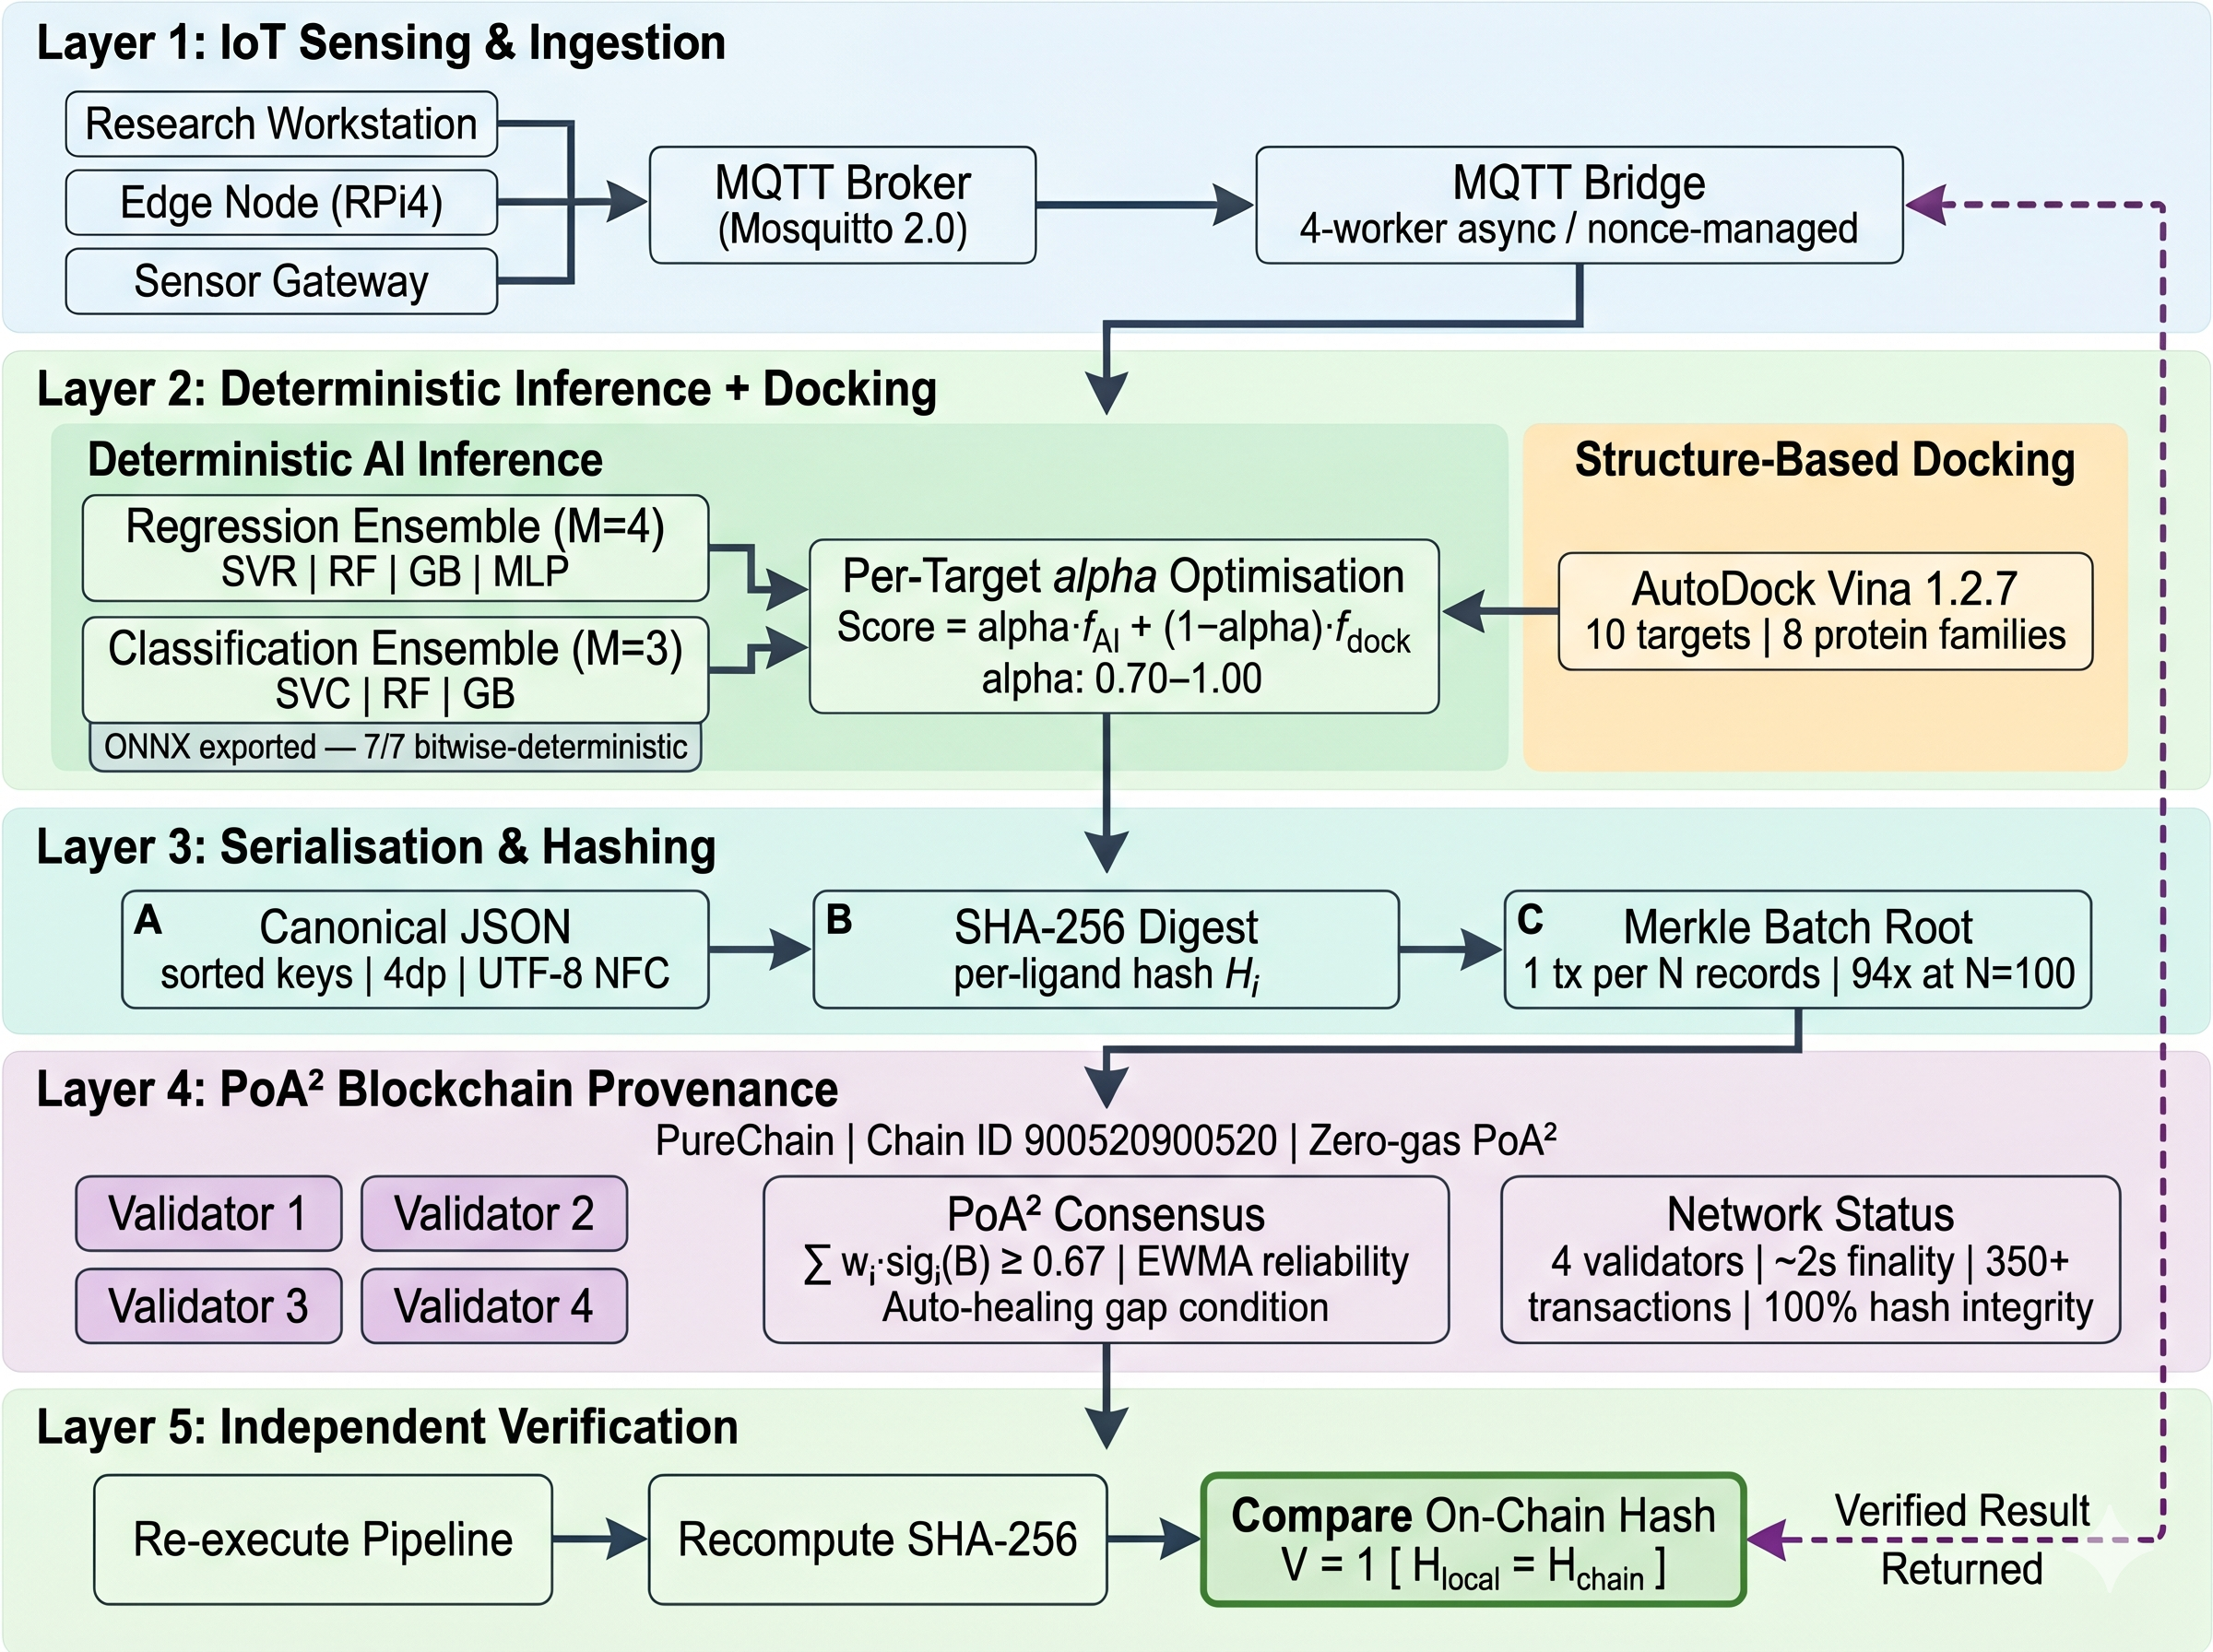
\includegraphics[width=0.60\textwidth]{images/system.png}
\caption{System architecture of PureProtX showing the five-layer 
pipeline for IoT-distributed verifiable scientific screening: 
(1)~IoT sensing and MQTT ingestion across heterogeneous edge nodes; 
(2)~deterministic dual-ensemble AI inference with ONNX-exported 
models and per-target $\alpha$-optimised AI--docking consensus fusion; 
(3)~canonical JSON serialisation with SHA-256 hashing and Merkle 
batch anchoring; (4)~PoA$^2$ blockchain provenance via PureChain 
across four live validators with auto-healing gap condition; and 
(5)~independent cryptographic verification by on-chain hash 
comparison. The dashed return path closes the end-to-end trust loop, 
delivering a verified result to the originating IoT node.}
\label{fig:system}
\end{figure*}

In parallel, edge- and IoT-oriented healthcare systems have shown how intelligent computation can be moved closer to data sources to reduce latency, communication load, and response time. Authors~\cite{alabdulatif2019secure} introduced a secure Edge-of-Things healthcare surveillance framework that combines distributed clustering with fully homomorphic encryption to preserve privacy during local analysis of biosignal data. Authors~\cite{muhammad2019computing} proposed an edge--cloud pathology detection framework in which EEG signals are preprocessed at the edge before cloud-side deep learning classification. Authors~ \cite{hossain2020deep} later extended this direction using MEC, CNN-based pathology detection, and network-level orchestration mechanisms such as SDN, network slicing, and self-organizing networks. Authors~\cite{ning2020mobile} formulated MEC-enabled 5G health monitoring for IoMT as cooperative and non-cooperative games that jointly optimize medical criticality, age of information, and energy consumption. While these works are strong in deployment, privacy, or scheduling terms, they do not jointly address deterministic scientific replay, canonical result hashing, and permissioned immutable verification of inference outputs.

At the application layer, recent virtual screening frameworks have dramatically improved the scale and practical effectiveness of computational hit discovery. Deep Docking demonstrated that neural prioritization can reduce the need for exhaustive docking of ultra-large libraries while preserving most of the high-value candidates \cite{gentile2022artificial}. More recently, RosettaVS/OpenVS combined physics-based docking, receptor flexibility, and active learning into a scalable AI-accelerated virtual screening platform capable of screening multi-billion compound libraries with experimentally validated hits \cite{zhou2024artificial}. Likewise, machine learning-guided docking with conformal prediction has shown that multi-billion-scale screening campaigns can be reduced by orders of magnitude while retaining many top-scoring candidates \cite{luttens2025rapid}. However, these systems treat screening output primarily as a ranking or discovery artifact rather than as a deterministic computational claim requiring cryptographically auditable replay. Therefore, the central gap that remains is the lack of an integrated framework that combines deterministic inference, hybrid AI--docking screening, canonical serialization, cryptographic hashing, edge-capable deployment, and permissioned blockchain-based verification. PureProtX is designed to address this gap by unifying these capabilities into a single end-to-end framework for verifiable IoT-distributed scientific computation.



\section{\textbf{system architecture and methodology}}
\label{sec:methods}


\subsection{\textbf{Architecture Overview}}
\label{sec:arch}

PureProtX is designed as a verifiable deterministic computation
framework for IoT-distributed scientific pipelines, instantiated here
on the drug-discovery workload of virtual compound screening.
\textcolor{black}{The screening workload serves as a concrete,
scientifically demanding demonstrator; the framework's
contribution is the verifiable-re-execution infrastructure
itself, which applies to any workload meeting the
requirements set out in Section~\ref{sec:generalization}.}
The system addresses a fundamental challenge in distributed scientific
IoT deployments: ensuring that inference results produced across
heterogeneous edge nodes are provably identical, tamper-evident,
and independently verifiable---properties that neither containerised
reproducibility frameworks nor conventional blockchain provenance
systems jointly provide.

The framework integrates five modular components into a unified
pipeline (Fig.~\ref{fig:system}):

\begin{enumerate}
    \item \textbf{IoT Ingestion Layer:} An MQTT pub/sub bridge that
    accepts compound batches from IoT sensing nodes and dispatches
    them to the inference pipeline via concurrent worker threads.
    \item \textbf{Deterministic AI Inference:} A dual consensus
    ensemble (four regression and three classification models) with
    fixed random seeds and canonical serialisation, producing
    bitwise-identical outputs across executions.
    \item \textbf{Structure-Based Docking:} AutoDock Vina~\cite{eberhardt2021autodock}
    providing physics-based binding affinity estimates, fused with
    AI scores through per-target optimised hybrid weighting.
    \item \textbf{Deterministic Serialisation:} All outputs are
    canonically serialised to JSON with lexicographically ordered
    keys, fixed numeric precision, and NFC-normalised encoding,
    then hashed via SHA-256.
    \item \textbf{PoA$^2$ Blockchain Provenance:} All pipeline digests
    are committed to PureChain, a live permissioned ledger with
    four active validators, enabling any party to independently
    verify result integrity by re-execution and on-chain comparison.
\end{enumerate}

The modular design ensures that each component can be executed,
tested, and verified independently.
Fig.~\ref{fig:system} illustrates the end-to-end data flow from
IoT ingestion through on-chain audit.
The complete pipeline is orchestrated through a command-line
interface described in Section~\ref{clidesign}.
\textcolor{black}{The individual building blocks---ONNX export,
canonical JSON, SHA-256, Merkle batching, MQTT ingestion,
and a permissioned ledger---are established primitives.
PureProtX composes them so that a result produced on one
edge node can be re-executed on another and proven
byte-identical against an on-chain record: a property
reproducibility frameworks and provenance ledgers do not
provide alone. Achieving it requires pinning the model
artifact and exact runtime configuration on which
determinism depends (Section~\ref{sec:onnx-results}), not
only the result digest.}

%%% ============================================================
%%% III-B  IoT DEPLOYMENT ARCHITECTURE
%%% ============================================================
\subsection{\textbf{IoT Deployment Architecture}}
\label{sec:iot-arch}

\subsubsection{Network Topology}

PureProtX is designed for deployment across a consortium of
institutional edge nodes, each contributing to both computation
and consensus. Layer 1 in
Fig.~\ref{fig:system} illustrates the target deployment topology:
IoT sensing nodes at research sites publish compound batches via
MQTT to a gateway-class edge node running the PureProtX inference
pipeline; the resulting digests are committed to PureChain across
a distributed PoA$^2$ validator network spanning institutional
boundaries.

\textcolor{black}{Hardware requirements are modest. On the real
edge devices evaluated (Section~\ref{sec:edge-results}), the
full pipeline---including the largest target, hERG---runs
within the memory of a Raspberry Pi~4 (4~GB), with peak
resident memory well below capacity. Larger available memory
and additional cores, as on the Jetson Orin Nano, improve
throughput but are not required for correctness.}

\subsubsection{MQTT Ingestion Bridge}
\label{sec:mqtt}

IoT devices submit compound batches to the PureProtX pipeline
via the MQTT protocol~\cite{mqtt5}, the standard lightweight
pub/sub transport for constrained IoT nodes.
The bridge subscribes to the \texttt{pureprot/compounds/ingest}
topic and processes incoming messages through a four-worker
\texttt{ThreadPoolExecutor}, enabling concurrent inference while
serialising blockchain commits through a thread-safe nonce manager.

Message schema (ingest):
\begin{equation*}
\{\,\texttt{job\_id},\; \texttt{target},\;
   \texttt{smiles}: [\ldots],\;
   \texttt{requester\_node}\,\}
\end{equation*}

For each received batch the bridge executes the following
atomic sequence: (i)~deserialise and validate the payload;
(ii)~run the deterministic consensus inference pipeline;
(iii)~serialise results to canonical JSON and compute SHA-256;
(iv)~commit digest to PureChain via the nonce-managed
transaction interface; (v)~publish ranked hits and the
on-chain audit digest to \texttt{pureprot/compounds/results}
and \texttt{pureprot/audit/hashes} respectively.

The nonce manager maintains a local atomic counter protected
by \texttt{threading.Lock}, eliminating the nonce-collision
failure mode that arises when concurrent threads independently
query \texttt{eth\_getTransactionCount}.
This recovers 100\% blockchain commit success under
four-worker concurrency, as validated in
Section~\ref{sec:mqtt-results}.

\subsubsection{Edge Deployment and Resource Characterisation}
\label{sec:edge-deploy}

\textcolor{black}{To characterize viability on real edge hardware,
experiments were conducted on two physical ARM devices---a
Raspberry Pi~4 Model~B (quad-core Cortex-A72, 4~GB) and an
NVIDIA Jetson Orin Nano (six-core Cortex-A78AE, aarch64)---with
an uncapped x86\_64 Linux host as the server reference
(Table~\ref{tab:edge-tiers}). Each device runs the complete
PureProtX inference pipeline: RDKit featurization, sklearn
consensus inference, canonical serialization, SHA-256 hashing,
and PureChain transaction submission. The x86\_64 reference is
a real, uncapped host, not a resource-limited container.}

\begin{table}[!t]
\centering
\caption{\textcolor{black}{real edge hardware used for evaluation
(no resource caps).}}
\label{tab:edge-tiers}
\scalebox{0.82}{
\textcolor{black}{%
\begin{tabular}{lllc}
\toprule
\textbf{Device} & \textbf{CPU} & \textbf{RAM} & \textbf{Role} \\
\midrule
x86\_64 host       & Multi-core x86\_64        & --       & Server reference \\
Jetson Orin Nano   & 6$\times$ Cortex-A78AE     & 8~GB     & GPU-class edge \\
Raspberry Pi~4     & 4$\times$ Cortex-A72       & 4~GB     & CPU-only edge \\
\bottomrule
\end{tabular}}}
\end{table}

%%% ============================================================
%%% III-C  DATA PREPARATION AND CURATION
%%% ============================================================
\subsection{\textbf{Data Preparation and Curation}}
\label{sec:data}

The virtual screening workload used to benchmark the IoT
infrastructure spans 10~therapeutically relevant protein targets
across 8~protein families (Table~\ref{tab:targets}).
This diversity ensures that infrastructure results are not
artefacts of a single target's characteristics.

\subsubsection{Target Selection}
The panel includes three HIV-1 antiviral targets representing
distinct stages of viral replication: protease
(CHEMBL243~\cite{ebiTargetHumanProt}), reverse transcriptase
(CHEMBL247~\cite{ebiTargetHuman}), and integrase
(CHEMBL3471~\cite{ebiTargetHumanInte}), providing a rigorous
intra-virus benchmark.
The remaining seven targets cover kinases (VEGFR2, CHEMBL279),
GPCRs (adenosine~A$_{2a}$, CHEMBL251; dopamine~D$_2$, CHEMBL217),
nuclear receptors (ER$\alpha$, CHEMBL1862; PPAR$\gamma$,
CHEMBL4005), a membrane protein (amyloid-$\beta$~A4,
CHEMBL2487~\cite{ebiTargetAmyloidbeta}), and an ion channel
(hERG, CHEMBL240).
Dataset sizes range from 999 (CHEMBL2487) to 16{,}640 (CHEMBL240)
compounds, totalling 71{,}853 molecules.
The hERG target (322~MB model, 16{,}640 compounds) additionally
serves as the stress-test case for edge resource evaluation.

\begin{table}[!t]
\centering
\caption{Ten-target benchmark panel. Splits are 60/20/20
train/validation/test (\texttt{random\_state=42}).
Active threshold: pIC$_{50} \geq 6.0$.}
\label{tab:targets}
\scalebox{0.72}{
\begin{tabular}{@{}llllrrrr@{}}
\toprule
\textbf{ChEMBL ID} & \textbf{Target} & \textbf{Family}
  & \textbf{PDB} & \textbf{N}
  & \textbf{Train} & \textbf{Val} & \textbf{Test} \\
\midrule
CHEMBL243  & HIV-1 Protease   & Viral protease   & 1HXW & 3{,}444  & 2{,}066 & 689   & 689 \\
CHEMBL247  & HIV-1 RT         & Viral polymerase & 3QIP & 10{,}308 & 6{,}184 & 2{,}062 & 2{,}062 \\
CHEMBL3471 & HIV-1 Integrase  & Viral integrase  & 3APF & 7{,}879  & 4{,}727 & 1{,}576 & 1{,}576 \\
CHEMBL279  & VEGFR2 (KDR)     & Kinase           & 3VHE & 14{,}008 & 8{,}404 & 2{,}802 & 2{,}802 \\
CHEMBL251  & Adenosine A$_{2a}$ & GPCR           & 4EIY & 2{,}126  & 1{,}275 & 425   & 426 \\
CHEMBL217  & Dopamine D$_2$   & GPCR             & 6CM4 & 1{,}570  & 942   & 314   & 314 \\
CHEMBL1862 & ER$\alpha$       & Nuclear receptor & 3ERT & 5{,}156  & 3{,}093 & 1{,}031 & 1{,}032 \\
CHEMBL4005 & PPAR$\gamma$     & Nuclear receptor & 2PRG & 9{,}723  & 5{,}833 & 1{,}945 & 1{,}945 \\
CHEMBL2487 & Amyloid-$\beta$ A4 & Membrane protein & 4IVT & 999    & 599   & 200   & 200 \\
CHEMBL240  & hERG             & Ion channel      & 5VA1 & 16{,}640 & 9{,}984 & 3{,}328 & 3{,}328 \\
\midrule
\multicolumn{4}{l}{\textbf{Total}} & \textbf{71{,}853} & & & \\
\bottomrule
\end{tabular}}
\end{table}

\subsubsection{Ligand Curation and Representation}
Bioactivity data were obtained from ChEMBL~v34~\cite{mendez2019chembl}
via the \texttt{chembl\_webresource\_client} API.
Only entries with explicit IC$_{50}$ or K$_i$ measurements in
nM were retained; ambiguous records were discarded and duplicates
resolved by median aggregation.
Activities were converted to the pIC$_{50}$ scale (Eq.~\ref{eq:pic50})
to stabilise variance and align with standard QSAR conventions.
Compounds were filtered by Lipinski's Rule of
Five~\cite{lipinski2004lead}, and all SMILES strings were
canonicalised using RDKit with deterministic atom ordering.
\begin{equation}
\label{eq:pic50}
\mathrm{pIC_{50}} = -\log_{10}(\mathrm{IC_{50}} \times 10^{-9}).
\end{equation}

Each ligand was represented as a hybrid descriptor
$\mathbf{x} \in \{0,1\}^{2048} \oplus \mathbb{R}^{10}$
comprising a 2{,}048-bit Morgan fingerprint (radius~2) and
ten physicochemical descriptors: molecular weight, LogP,
hydrogen-bond donors and acceptors, TPSA, rotatable bonds,
aromatic ring count, fraction~$sp^3$, heavy atom count, and
formal charge---yielding a 2{,}058-dimensional feature vector.
Curated datasets were split 60/20/20 into training, validation,
and test sets using a fixed random seed (\texttt{random\_state=42}).
The validation set is used exclusively for hyperparameter
selection and $\alpha$~optimisation; the test set is held out
for all reported metrics.
All curation scripts, version-pinned dependencies, and example
deterministic JSON outputs are available in the public
PureProtX repository.\footnote{\url{https://github.com/xaviwho/PureProt}}

\subsubsection{Docking Preparation}
Receptors were curated from high-resolution PDB structures
(Table~\ref{tab:targets}), with crystallographic waters removed,
polar hydrogens added, and Gasteiger charges assigned before
conversion to PDBQT format using meeko~0.7.1 and gemmi~0.7.4.
Ligands were protonated at pH~7.4, minimised using MMFF94, and
converted to PDBQT.
Grid boxes were centred on co-crystallised ligands and extended
by 5~\AA.

%%% ============================================================
%%% III-D  DETERMINISTIC AI INFERENCE MODULE
%%% ============================================================
\subsection{\textbf{Deterministic AI Inference Module}}
\label{sec:ai}

\subsubsection{Design Rationale: Classical ML for Bitwise Determinism}

A core requirement of the PureProtX infrastructure is that
any re-execution of the pipeline on any node produces
bit-for-bit identical outputs, enabling SHA-256 digest
comparison against the on-chain record.
This requirement mandates the use of classical ML rather
than GPU-accelerated deep learning: non-deterministic
floating-point reduction orders in CUDA kernels make
bitwise reproducibility across executions impossible
without hardware-specific constraints~\cite{heumos2023mlf}.
All seven models are trained with fixed random seeds
(\texttt{random\_state=42}) and exported to ONNX format
via \texttt{skl2onnx}. \textcolor{black}{As characterized in
Section~\ref{sec:onnx-results}, this yields bitwise
determinism within a pinned runtime configuration across
heterogeneous platforms, rather than an unconditional
cross-platform guarantee.}

\subsubsection{Dual Ensemble Architecture}
PureProtX employs two complementary ensembles for
binding-affinity estimation.
The \emph{regression ensemble} comprises four models:
SVR, RF, GB, and MLP, each trained to predict continuous
pIC$_{50}$ values.
The consensus regression prediction is the arithmetic
mean across the $M{=}4$ regressors:
\begin{equation}
\label{eq:consensus-reg}
\hat{y}_{\mathrm{cons}}(\mathbf{x})
  = \frac{1}{M}\sum_{m=1}^{M}\hat{y}_m(\mathbf{x}).
\end{equation}

The classification ensemble comprises three models:
SVC, RF, and GB, trained to discriminate active
(pIC$_{50} \geq 6.0$) from inactive compounds.
Individual class probabilities are averaged to form the
consensus classification score, which is subsequently
calibrated via isotonic regression to ensure monotonic
alignment with observed activity rates.
The calibrated classification output serves as
$f_{\mathrm{AI,clf}}$, while the regression consensus
(after isotonic calibration) serves as
$f_{\mathrm{AI,reg}}$.

\subsubsection{Hyperparameter Tuning}
Hyperparameters were optimised on the validation set
(no test-set leakage) via grid search:
\begin{itemize}
    \item \textbf{SVR/SVC:} $C \in \{0.1, 1, 10\}$,
    $\gamma \in \{\mathrm{scale}, 0.01\}$ (6~configurations).
    For datasets exceeding 3{,}000 samples, tuning uses
    a 3{,}000-compound random subsample (fixed seed) to
    manage $O(n^2)$ kernel complexity.
    \item \textbf{RF/GB:} \texttt{n\_estimators}
    $\in \{100, 200\}$, \texttt{max\_depth}
    $\in \{\mathrm{None}, 10, 20\}$ (6~configurations each).
\end{itemize}
Best configurations were selected by validation-set BEDROC
(classification) or $R^2$ (regression).
The full deterministic training workflow is provided
in Algorithm~\ref{alg:ensemble}.

\subsubsection{Cross-Platform Determinism via ONNX Export}
\label{sec:onnx}

\textcolor{black}{To characterize determinism across heterogeneous IoT
deployments, all seven} trained models are exported to the ONNX format using
\texttt{skl2onnx} (opset 15).
\textcolor{black}{ONNX inference via \texttt{onnxruntime} is
bitwise-deterministic within a pinned runtime configuration---a
fixed ONNX Runtime version and intra-op thread count---rather
than universally across all platforms. PureProtX pins and
anchors this configuration on-chain so that any verifier
reproduces the exact conditions under which a result was
produced. The extent of cross-version, cross-thread, and
cross-architecture determinism is characterized empirically
in Section~\ref{sec:onnx-results}.}

Each ONNX model binary is hashed via SHA-256 and the digest
committed to PureChain, anchoring the exact inference
artefact to an immutable on-chain record.
Any deployment node can verify that it is running the
authorised model version by comparing its local ONNX hash
against the on-chain value.
\textcolor{black}{The SVR is exported via the float32 kernel path,
as ONNX Runtime provides no double-precision \texttt{SVMRegressor}
kernel; the resulting sklearn-to-ONNX concordance, and its
architecture-dependence, are characterized in
Section~\ref{sec:onnx-results}.}

\begin{algorithm}[!htbp]
\scriptsize
\caption{Consensus AI Ensemble Training}
\label{alg:ensemble}
\KwData{Dataset $D = \{(\mathbf{x}_i, y_i)\}_{i=1}^n$,
  $\mathbf{x}_i \in \{0,1\}^{2048} \oplus \mathbb{R}^{10}$,
  $y_i \in \mathbb{R}$}
\KwResult{Trained models $\mathcal{M}_{\mathrm{reg}}^*$,
  $\mathcal{M}_{\mathrm{clf}}^*$; ONNX exports;
  on-chain hashes $\{H(m^*)\}$}
Split $D$ into Train (60\%), Val (20\%), Test (20\%)
  with \texttt{random\_state=42}\;
Standardise features using training-set statistics\;
\BlankLine
\textbf{Regression ensemble} ($M = 4$: SVR, RF, GB, MLP):\;
\For{each model $m \in \mathcal{M}_{\mathrm{reg}}$}{
    Grid search on Val; select $\theta_m^*$
      $= \arg\max_\theta R^2_{\mathrm{val}}$\;
    Retrain $m^*$ on Train with $\theta_m^*$\;
    Export to ONNX; compute $H(m^*)
      = \mathrm{SHA256}(\mathrm{ONNX}(m^*))$\;
    Log $H(m^*)$ to PureChain\;
}
Consensus: $\hat{y}_{\mathrm{cons}}(\mathbf{x})
  = \frac{1}{M}\sum_{m=1}^{M} \hat{y}_m(\mathbf{x})$\;
Apply isotonic calibration on Val
  $\Rightarrow f_{\mathrm{AI,reg}}$\;
\BlankLine
\textbf{Classification ensemble} ($M = 3$: SVC, RF, GB):\;
Binarise labels: active if $y_i \geq 6.0$\;
\For{each model $m \in \mathcal{M}_{\mathrm{clf}}$}{
    Grid search on Val using BEDROC criterion\;
    Export to ONNX; hash and log to PureChain\;
}
Consensus probability: $\hat{p}_{\mathrm{cons}}
  = \frac{1}{3}\sum_{m=1}^{3} \hat{p}_m$\;
Apply isotonic calibration on Val
  $\Rightarrow f_{\mathrm{AI,clf}}$\;
\BlankLine
\textbf{Evaluate on Test:}
  $R^2$, RMSE, AUC-ROC, AUC-PR, Brier score\;
\Return $\mathcal{M}_{\mathrm{reg}}^*$,
  $\mathcal{M}_{\mathrm{clf}}^*$,
  ONNX exports, $\{H(m^*)\}$\;
\end{algorithm}

%%% ============================================================
%%% III-E  DOCKING MODULE
%%% ============================================================
\subsection{\textbf{Docking Module}}
\label{sec:docking}

Structure-based docking was performed with AutoDock
Vina~1.2.7~\cite{eberhardt2021autodock} at
exhaustiveness$\,{=}\,4$ with up to 9 binding modes and
an energy range of 3.0~kcal/mol.
Raw binding energies $\Delta G_i$ were normalised via
z-scoring within each target:
\begin{equation}
\label{eq:fdock}
f_{\mathrm{dock}}(i)
  = \frac{\Delta G_i - \mu_{\Delta G}}{\sigma_{\Delta G}}.
\end{equation}
Docking scores were generated offline and cached per target.
The structural signal from Vina is partially independent
of the Morgan fingerprint features used by the AI models,
providing complementary information when the binding pocket
is sufficiently rigid for reliable rigid-receptor docking.

To justify exhaustiveness$\,{=}\,4$, we conducted a
sensitivity analysis comparing per-molecule scores at
$e{=}1$ and $e{=}4$ using Spearman rank correlation.
Mean $\rho = 0.809$ across 10 targets confirms rankings
are well-preserved; the two outliers (HIV-1~RT,
$\rho=0.688$; PPAR$\gamma$, $\rho=0.622$) correspond
exactly to targets where the $\alpha$ optimiser assigns
$\alpha=1.0$, automatically discarding unreliable
docking signals.
All docking results were serialised deterministically
and hashed on-chain (Algorithm~\ref{alg:docking}).

\begin{algorithm}[!htbp]
\scriptsize
\caption{Structure-Based Docking and Enrichment Evaluation}
\label{alg:docking}
\KwData{Receptor $P$ (PDB);
  Ligand library $\mathcal{L} = \{l_1, \ldots, l_n\}$}
\KwResult{Normalised scores $\{f_{\mathrm{dock}}(i)\}$;
  enrichment metrics; on-chain hash}
Prepare receptor: remove waters, add polar H,
  assign Gasteiger charges, convert to PDBQT\;
\For{each $l \in \mathcal{L}$}{
    Protonate at pH~7.4; minimise (MMFF94);
    convert to PDBQT\;
}
Centre grid on co-crystallised ligand $+ 5$~\AA\;
\For{each $l_i \in \mathcal{L}$}{
    $\Delta G_i \leftarrow \mathrm{Vina.dock}(P, l_i)$
      at $e{=}4$, modes${=}9$, range${=}3.0$\;
}
$f_{\mathrm{dock}}(i) = (\Delta G_i - \mu_{\Delta G})
  / \sigma_{\Delta G}$\;
Compute EF@$k$\% ($k \in \{1,5,10\}$) and BEDROC
  ($\alpha = 20$)\;
Convert results to canonical JSON;
  $H = \mathrm{SHA256}(\mathrm{JSON})$;
  log $H$ to PureChain\;
\Return $\{f_{\mathrm{dock}}(i)\}$, EF, BEDROC, $H$\;
\end{algorithm}

%%% ============================================================
%%% III-F  HYBRID CONSENSUS FUSION
%%% ============================================================
\subsection{\textbf{Hybrid AI--Docking Consensus Fusion}}
\label{sec:fusion}

Calibrated AI scores $f_{\mathrm{AI}}(i)$ and normalised
docking scores $f_{\mathrm{dock}}(i)$ are fused through
a convex weighting:
\begin{equation}
\label{eq:hybrid}
\mathrm{Score}_{\mathrm{final}}(i)
  = \alpha \, f_{\mathrm{AI}}(i)
  + (1 - \alpha)\, f_{\mathrm{dock}}(i),
\qquad \alpha \in [0, 1].
\end{equation}
The parameter $\alpha$ is optimised per target on the
validation set by grid search over
$\alpha \in \{0.00, 0.05, \ldots, 1.00\}$ (21~values),
maximising BEDROC.
Ranking ties are resolved by secondary sorting on
regression pIC$_{50}$, ensuring deterministic rank ordering.

LOTO cross-validation over the
nine remaining per-target optima provides a recommended
global weight ($\bar{\alpha}_{\mathrm{LOTO}} \pm \mathrm{SD}$)
for deployment on novel targets without per-target
optimisation.
The contribution of the hybrid module is characterised
as a systematic analysis of \emph{when} structure-based
docking adds value over ligand-only AI prediction,
rather than a claim of universal superiority.
All fusion outputs are serialised and hashed on-chain
(Algorithm~\ref{alg:consensus}).

\begin{algorithm}[!htbp]
\scriptsize
\caption{Consensus AI--Docking Fusion}
\label{alg:consensus}
\KwData{Calibrated AI scores $\{f_{\mathrm{AI}}(i)\}$;
  normalised docking scores $\{f_{\mathrm{dock}}(i)\}$;
  Validation set $\mathcal{V}$}
\KwResult{Final scores $\{\mathrm{Score}_{\mathrm{final}}(i)\}$;
  optimal $\alpha^*$; on-chain hash}
\textbf{Alpha optimisation on $\mathcal{V}$:}\;
\For{each $\alpha \in \{0.00, 0.05, \ldots, 1.00\}$}{
    $\mathrm{Score}_\alpha(i) = \alpha \cdot f_{\mathrm{AI}}(i)
      + (1-\alpha) \cdot f_{\mathrm{dock}}(i)$\;
    Rank by $\mathrm{Score}_\alpha$;
    compute BEDROC$(\alpha)$\;
}
$\alpha^* = \arg\max_\alpha \mathrm{BEDROC}(\alpha)$\;
Score test set using $\alpha^*$; rank all ligands\;
\textbf{LOTO generalisation:}\;
\For{each held-out target $t$}{
    $\alpha_{\mathrm{LOTO}}^{(t)}
      = \mathrm{mean}(\alpha^*_{j \neq t})$\;
}
Report $\bar{\alpha}_{\mathrm{LOTO}} \pm \mathrm{SD}$\;
$H(\mathcal{J}) = \mathrm{SHA256}(\mathcal{J})$;
log to PureChain\;
\Return $\{\mathrm{Score}_{\mathrm{final}}(i)\}$,
  $\alpha^*$, $\bar{\alpha}_{\mathrm{LOTO}}$,
  $H(\mathcal{J})$\;
\end{algorithm}

%%% ============================================================
%%% III-G  PoA² BLOCKCHAIN PROVENANCE LAYER
%%% ============================================================
\subsection{\textbf{PoA$^2$ Blockchain Provenance Layer}}
\label{sec:blockchain}

\subsubsection{PureChain Network}

PureProtX anchors all pipeline outputs to PureChain, a
live permissioned ledger (Chain ID 900520900520)
\textcolor{black}{built on a Proof-of-Authority (Clique) network, over
which the PoA$^2$ reliability and gap-condition mechanism is
defined~\cite{kim2025proof, ajakwe2025ebctc}.}
PureChain operates with four active validators (Table~IV),
\textcolor{black}{whose addresses were recovered from block-seal
attribution.} The $\sim$2 s consensus latency—orders of magnitude
above local in-process hashing—confirms that transactions pass
through genuine multi-validator block sealing rather than a
single-node database.

\begin{figure}[!t]
\centering
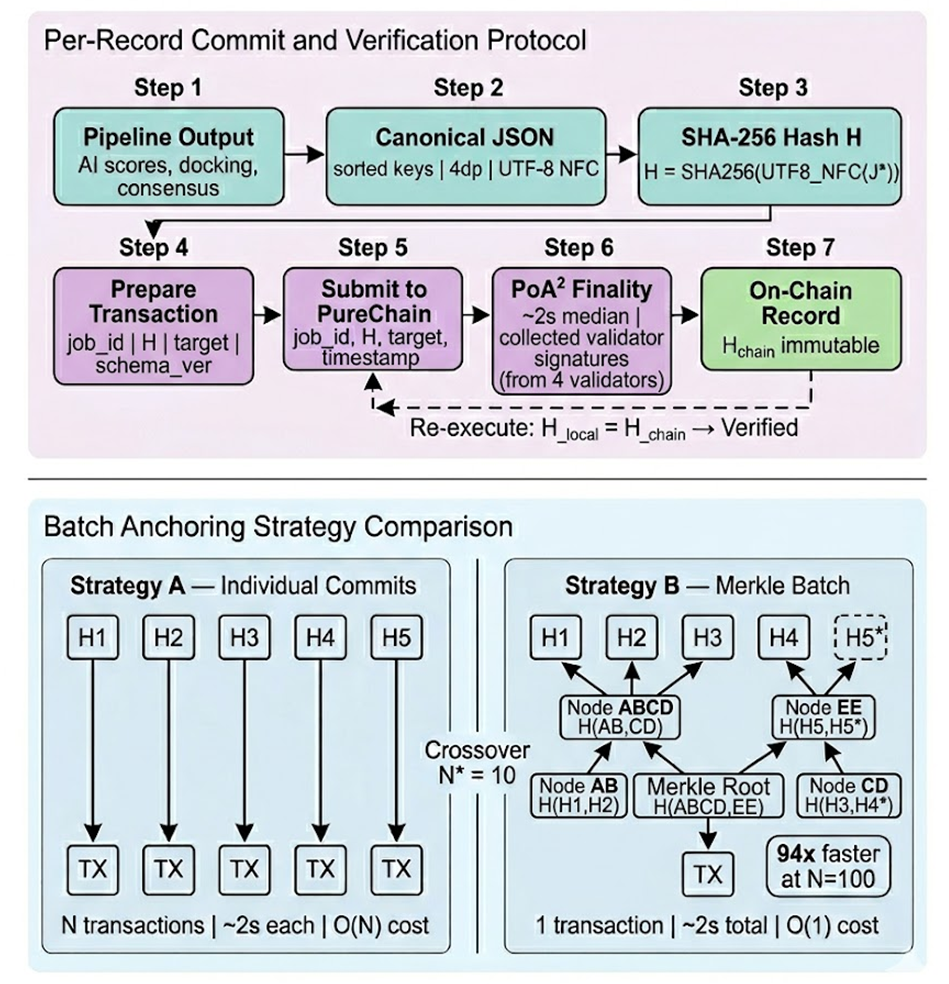
\includegraphics[width=0.85\columnwidth]{images/poa-provenance.png}
\caption{PoA$^2$ blockchain provenance layer in PureProtX.
\textit{Top:} Per-record commit and verification protocol ---
pipeline outputs are canonically serialised, hashed via SHA-256,
and submitted to PureChain; PoA$^2$ finality is reached when
weighted validator signatures satisfy
$\sum w_i \cdot \mathrm{sig}_i(B) \ge 0.67$ across four
active validators (${\sim}2$~s median). Any party can
re-execute the pipeline and compare $H_{\mathrm{local}}$
against $H_{\mathrm{chain}}$ for independent cryptographic
verification.
\textit{Bottom:} Merkle batch anchoring (Strategy~B) reduces
anchoring cost from $O(N)$ transactions to $O(1)$, with
crossover at $N^*{=}10$ and a 94$\times$ speedup at
$N{=}100$ relative to per-record commits (Strategy~A).
H5$^*$ denotes the odd-leaf duplication convention.}
\label{fig:poa-provenance}
\end{figure}

\begin{table}[!t]
\centering
\caption{Live PureChain validator set queried at
  block~1{,}012{,}544.}
\label{tab:validators}
\scalebox{0.78}{
\begin{tabular}{ll}
\toprule
\textbf{Validator} & \textbf{Address} \\
\midrule
Validator~1 & \texttt{0x03df376cd39dd1706a903126dbc382846db16929} \\
Validator~2 & \texttt{0x5b7a1a9b6b4500c3f1ff359dc217f374aa59ddb1} \\
Validator~3 & \texttt{0x82293aec2dd5816a1d88b9a15b645e018b5b7e1e} \\
Validator~4 & \texttt{0xc6a79c2d19944574372c64b6bf28551832b2b1f9} \\
\midrule
\multicolumn{2}{l}{Connected peers: 5 \;|\;
  Active signers observed: 3 of 4} \\
\bottomrule
\end{tabular}}
\end{table}

\subsubsection{PoA$^2$ Consensus Protocol}

In PoA$^2$, block acceptance requires that the weighted
sum of validator signatures satisfies:
\begin{equation}
\label{poa}
\sum_{i=1}^{N_a} w_i \cdot \mathrm{sig}_i(B) \ge \theta,
\end{equation}
where $N_a$ is the number of active authorities,
$w_i$ is the trust weight of validator~$i$, and $\theta$
is the consensus threshold (typically 0.67).

Validator reliability is tracked via an exponentially
weighted moving average (EWMA):
\begin{equation}
\label{validator}
R_i(t) =
\frac{\sum_{k=1}^{N}\gamma^{N-k}s_i(k)}
     {\sum_{k=1}^{N}\gamma^{N-k}},
\end{equation}
where $s_i(k)=1$ if validator~$i$ signed block~$k$,
and $\gamma$ favours recent participation.
Validators with declining reliability are demoted to
standby; standby nodes with consistent uptime are promoted.

The gap condition enforces a healthy validator set:
\begin{equation}
\label{eq:gap}
\max_{j\in S}[R_j] - \min_{i\in A}[R_i] < \Delta_R.
\end{equation}
If violated, the least reliable active node is replaced
by the most reliable standby node, providing self-healing
fault tolerance without a central authority.

The observed signer rotation (3 of 4 validators signing
recent blocks) and $\sim$2~s consensus latency directly
reflect this multi-validator architecture.
\textcolor{black}{The production PureChain deployment is a
permissioned Proof-of-Authority (PoA) network built on
go-ethereum (Clique). We therefore present the PoA$^2$
reliability weighting and gap condition
(Eq.~\ref{poa}--\ref{eq:gap}) as a \emph{proposed
control-layer mechanism} that operates over such a
permissioned deployment through the standard signer-voting
interface, rather than as a modification of the underlying
node consensus. We validate this mechanism empirically via
controlled failure injection on a faithful four-signer
testnet built from the PureChain genesis configuration
(chain~ID~900520900520); the measured fault-tolerance
envelope and gap-condition recovery are reported in
Section~\ref{sec:consensus-results}.}

\subsubsection{Deterministic Serialisation}

All screening outputs are serialised into a canonical JSON
object with lexicographically ordered keys, fixed numeric
precision (4~d.p., round-half-even), NFC-normalised UTF-8
encoding, and explicit provenance fields (software versions,
random seeds, schema version).
The SHA-256 digest constitutes the committed hash:
\begin{equation}
\label{eq:hash}
H = \mathrm{SHA256}\!\bigl(\mathrm{UTF8\_NFC}(J^\star)\bigr),
\qquad
V = \mathbf{1}[H = H_{\mathrm{chain}}].
\end{equation}
Verification succeeds if and only if the locally recomputed
digest matches the immutable on-chain record.

\subsubsection{Merkle Batch Anchoring}

For batch IoT deployments, PureProtX computes per-ligand
hashes $\{H_i\}_{i=1}^N$ and combines them into a Merkle
root:
\begin{equation}
H_{\mathrm{batch}} = \mathrm{MerkleRoot}(H_1, \ldots, H_N),
\end{equation}
submitting a single blockchain transaction regardless of
batch size~$N$.
This reduces anchoring cost from $O(N)$ transactions to
$O(1)$, while preserving the ability to verify any
individual record in $O(\log N)$ time via a Merkle proof.
The scalability advantage is characterised empirically
in Section~\ref{sec:scalability-results}.

\subsubsection{On-Chain Commitment and Independent Verification}

Each blockchain transaction records
$\langle\texttt{job\_id},\, H,\, \texttt{target},\,
\texttt{schema\_ver},\, \texttt{timestamp}\rangle$
on PureChain.
Any party can independently verify a result by:
(i)~re-executing the deterministic pipeline with the
same inputs and configuration; (ii)~regenerating the
canonical JSON and computing its SHA-256 digest locally;
(iii)~querying the on-chain record and comparing digests.
A standalone verification script (\texttt{tools/verify\_onchain.py})
is provided in the repository.
The blockchain audit workflow is illustrated in
Fig.~\ref{fig:poa-provenance}.

%%% ============================================================
%%% III-H  CLI PROTOCOL
%%% ============================================================
\subsection{\textbf{CLI Protocol Design}}
\label{clidesign}

The PureProtX command-line interface provides the unified
orchestration layer enforcing a standardised execution
protocol: identical commands and configurations yield
byte-for-byte identical outputs, allowing results to be
independently regenerated and verified against on-chain
records.

The CLI exposes seven modular commands:
\begin{enumerate}
    \item \textbf{\texttt{pureprot fetch-data}:}
    Downloads and preprocesses ligand--target bioactivity data.
    \item \textbf{\texttt{pureprot train-model}:}
    Trains the dual ensemble, exports ONNX artefacts,
    and logs model hashes to PureChain
    (Algorithm~\ref{alg:ensemble}).
    \item \textbf{\texttt{pureprot dock}:}
    Runs structure-based docking with AutoDock Vina
    (Algorithm~\ref{alg:docking}).
    \item \textbf{\texttt{pureprot consensus}:}
    Fuses AI and docking scores via per-target $\alpha$
    optimisation (Algorithm~\ref{alg:consensus}).
    \item \textbf{\texttt{pureprot screen}:}
    Runs the end-to-end virtual screening pipeline.
    \item \textbf{\texttt{pureprot verify}:}
    Validates a batch of molecules from a CSV file.
    \item \textbf{\texttt{pureprot history}:}
    Recomputes result hashes and compares them with
    on-chain digests.
\end{enumerate}

\begin{figure}[!htbp]
\centering
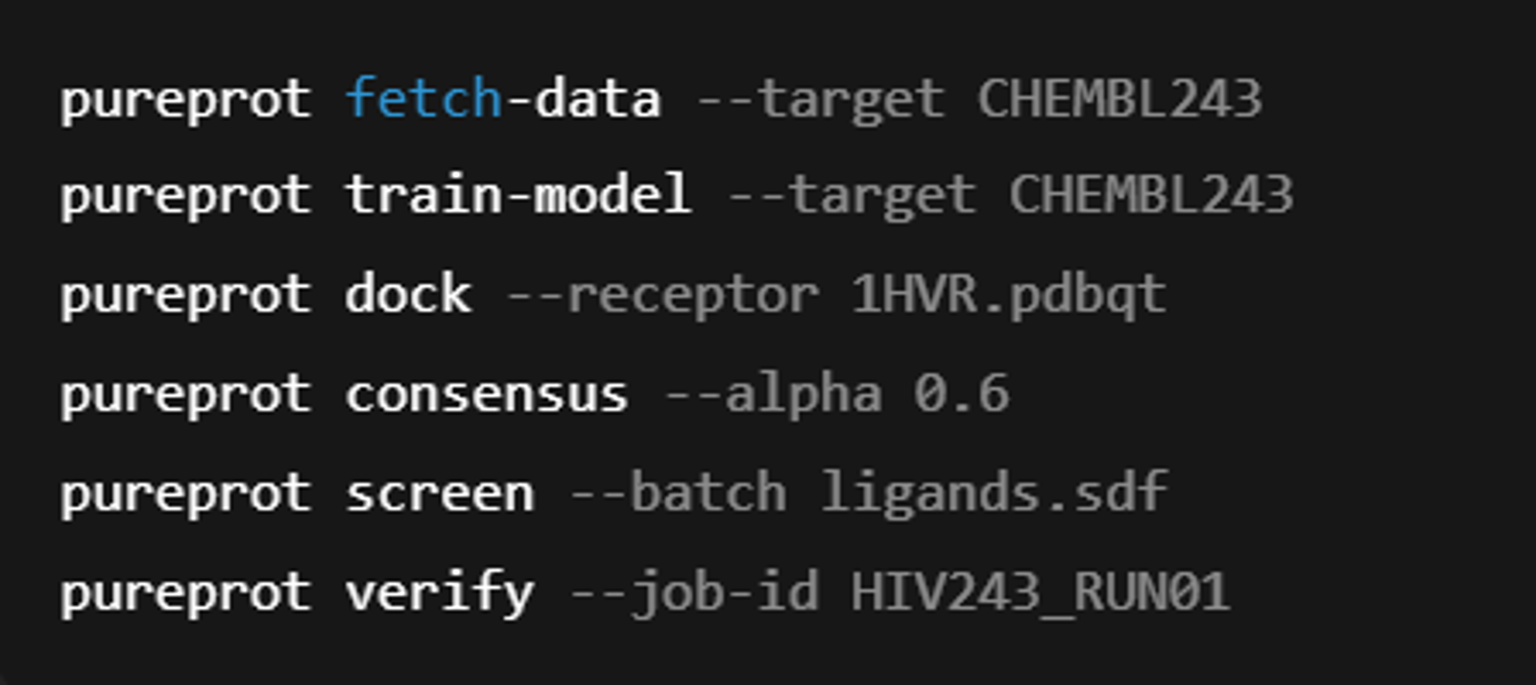
\includegraphics[width=0.45\textwidth]{images/cli.png}
\caption{A Complete PureProtX Workflow}
\label{fig:cli}
\end{figure}

All commands accept a YAML configuration file specifying
paths, model parameters, grid definitions, consensus
weights, and blockchain settings.
Strict parameter validation ensures deterministic
execution across heterogeneous environments.
A complete workflow from data acquisition to
blockchain-verified output is illustrated in
Fig.~\ref{fig:cli}.



%% ============================================================
%%  SYSTEM SETUP TABLE — PureProtX
%%  Place in Section IV: Experimental Setup
%%  Replace or supplement the existing prose description.
%% ============================================================

\begin{table}[!htbp]
\centering
\caption{PureProtX system setup and experimental configuration.}
\label{tab:system-setup}
\scalebox{0.72}{
\begin{tabular}{p{2.6cm} p{2.8cm} p{4.5cm}}
\toprule
\textbf{Component} & \textbf{Parameter} & \textbf{Value / Specification} \\
\midrule

\multirow{6}{*}{\textbf{Software Stack}}
  & Operating System      & Ubuntu 24.04 LTS (Docker container) \\
  & Python                & 3.12.10 \\
  & scikit-learn          & 1.8 (with \texttt{FrozenEstimator} for serialisation) \\
  & RDKit                 & 2025.9.4 \\
  & AutoDock Vina         & 1.2.7 \\
  & Web3.py               & 7.14.1 \\

\midrule
\multirow{4}{*}{\textbf{ONNX \& Determinism}}
  & skl2onnx              & 1.17.0 \\
  & onnxruntime           & 1.18.0 \\
  & ONNX opset            & 15 \\
  & Random seed           & \texttt{random\_state = 42} (all stochastic components) \\

\midrule
\multirow{5}{*}{\textbf{IoT Middleware}}
  & MQTT broker           & Eclipse Mosquitto 2.0 (Docker) \\
  & MQTT client           & paho-mqtt 2.0.0 \\
  & Bridge workers        & 4-worker \texttt{ThreadPoolExecutor} with nonce manager \\
  & Ingest topic          & \texttt{pureprot/compounds/ingest} \\
  & Results topic         & \texttt{pureprot/compounds/results} \\

\midrule
\multirow{6}{*}{\textbf{Blockchain}}
  & Network               & PureChain  \\
  & Chain ID              & 900520900520 \\
  & RPC endpoint          & \texttt{https://purechainnode.com} \\
 & Consensus             & \textcolor{black}{Permissioned PoA (Clique); PoA$^2$ control layer} \\
  & Active validators     & 4 (Clique, zero-gas) \\
  
\midrule
\multirow{4}{*}{\textbf{Serialisation}}
  & Format                & Canonical JSON \\
  & Key ordering          & Lexicographic \\
  & Numeric precision     & 4 decimal places (round-half-even) \\
  & Encoding              & UTF-8 NFC \\

\midrule
\multirow{3}{*}{\textcolor{black}{\textbf{Edge Hardware}}}
  & \textcolor{black}{Server reference} & \textcolor{black}{Uncapped x86\_64 Linux host} \\
  & \textcolor{black}{GPU-class edge}   & \textcolor{black}{NVIDIA Jetson Orin Nano (6$\times$Cortex-A78AE, 8~GB)} \\
  & \textcolor{black}{CPU-only edge}    & \textcolor{black}{Raspberry Pi~4 Model~B (4$\times$Cortex-A72, 4~GB)} \\

\midrule
\multirow{6}{*}{\textbf{Docking}}
  & Engine                & AutoDock Vina 1.2.7 \\
  & Exhaustiveness        & 4 \\
  & Binding modes         & 9 \\
  & Energy range          & 3.0~kcal/mol \\
  & Receptor preparation  & meeko~0.7.1 + gemmi~0.7.4 (PDBQT) \\
  & Ligand preparation    & MMFF94 minimisation; protonation at pH~7.4 \\

\midrule
\multirow{6}{*}{\textbf{ML Ensemble}}
  & Regression models     & SVR (RBF), Random Forest, Gradient Boosting, MLP ($M{=}4$) \\
  & Classification models & SVC, Random Forest, Gradient Boosting ($M{=}3$) \\
  & Calibration           & Isotonic regression (validation set) \\
  & Hyperparameter search & Grid search on validation set (no test-set leakage) \\
  & Feature vector        & 2{,}048-bit Morgan FP (radius~2) $\oplus$ 10 physicochemical
                           descriptors = 2{,}058 dimensions \\
  & Activity threshold    & pIC$_{50} \geq 6.0$ (active) \\

\midrule
\multirow{5}{*}{\textbf{Dataset}}
  & Source                & ChEMBL v34; DUD-E (external validation) \\
  & Targets               & 10 protein targets across 8 families \\
  & Total compounds       & 71{,}853 \\
  & Data split            & 60\% train / 20\% validation / 20\% test
                           (\texttt{random\_state=42}) \\
  & Filtering             & Lipinski Rule of Five; explicit IC$_{50}$ or
                           K$_i$ only; duplicates by median aggregation \\

\bottomrule
\end{tabular}}
\end{table}
\section{\textbf{experimental setup}}
\label{sec:experiments}
\textcolor{black}{Software components were developed and validated in a pinned
software environment (Table~V) to fix dependency versions for reproducibility.
Edge-performance and cross-architecture determinism experiments were then run
on real hardware---an uncapped x86\_64 server reference, an NVIDIA Jetson
Orin Nano, and a Raspberry Pi~4 (Table~II)---rather than in resource-capped
containers.} Table~V summarises the complete system configuration, software
stack, blockchain parameters, \textcolor{black}{edge hardware,} and dataset
specification. Blockchain operations used the PureChain
deployment (Chain ID 900520900520, zero-gas \textcolor{black}{permissioned
PoA}); all on-chain transactions are independently verifiable via
\texttt{tools/verify\_onchain.py}.

\section{\textbf{results and discussion}}
\label{sec:results}

This section evaluates PureProtX against the five modular
components described in Section~\ref{sec:methods}.
IoT infrastructure results are presented first
(Sections~\textcolor{black}{V-A–V-H}), covering edge deployment viability,
PoA$^2$ consensus performance and validator failure injection, MQTT
ingestion throughput, Merkle batch scalability, \textcolor{black}{alternative
provenance baselines,} cross-platform determinism, tamper detection, and
blockchain overhead. Screening workload results follow
(Sections~\textcolor{black}{V-I–V-M}), demonstrating that the infrastructure
sustains a computationally demanding and scientifically realistic application
across 10 protein targets\textcolor{black}{, and that the framework
generalizes beyond this workload}.
All blockchain experiments used the live PureChain
\textcolor{black}{deployment} (Chain ID 900520900520, RPC
\texttt{https://purechainnode.com}, zero-gas
\textcolor{black}{permissioned PoA}), with over 350 on-chain transactions
across blocks 1,010,803–1,012,680.



%%% ============================================================
%%% V-A  EDGE NODE PERFORMANCE  →  FIGURE
%%% ============================================================
\subsection{\textbf{Edge Node Performance}}
\label{sec:edge-results}

\begin{figure}[!htbp]
\centering
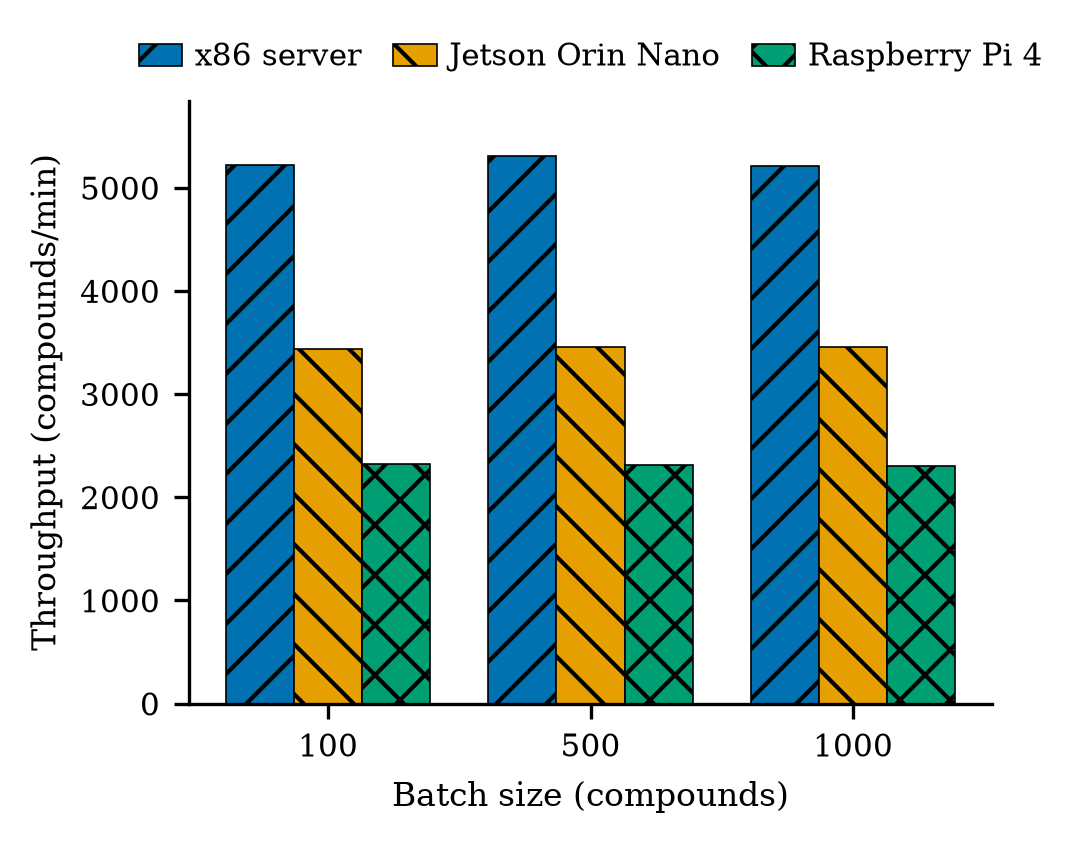
\includegraphics[width=\columnwidth]{images/fig2_edge_throughput.png}
\caption{\textcolor{black}{Measured screening throughput on
real hardware---x86\_64 server reference, Jetson Orin Nano, and
Raspberry Pi~4---across batch sizes $\{100,500,1000\}$. The x86
reference is an uncapped host, not a resource-limited container.
Throughput is stable across batch size on each device; all runs
achieved 100\% on-chain commit success.}}
\label{fig:edge}
\end{figure}

\textcolor{black}{Fig.~\ref{fig:edge} shows measured screening
throughput on the three real devices
(Table~\ref{tab:edge-tiers}) across batch sizes
$N \in \{100, 500, 1{,}000\}$. Throughput is stable across
batch size on each device. Relative to the x86\_64 server
reference, the Jetson Orin Nano sustains roughly two-thirds
and the Raspberry Pi~4 roughly two-fifths of server
throughput, giving a clear server$\rightarrow$Jetson$\rightarrow$Pi4
gradient. All runs achieved 100\% on-chain commit success.}

\textcolor{black}{On real hardware, peak resident memory remained
well within each device's capacity for all targets, including
the largest (hERG); we observed no out-of-memory failures.
This retracts our earlier simulation-based report of a
constrained-tier OOM, which was an artifact of an imposed
512~MB Docker cap rather than a property of real edge
hardware. The measured throughput gap across devices reflects
a genuine compute difference---inference accounts for the
majority of per-batch wall time on all three devices---rather
than the I/O-bound behavior suggested by the earlier
simulation. Both ARM devices comfortably sustain the full
pipeline, confirming edge-deployment viability on real
silicon.}


%%% ============================================================
%%% V-B  PoA² CONSENSUS LATENCY  →  TABLE
%%% ============================================================
\subsection{\textbf{PoA$^2$ Consensus Latency and Hash Integrity}}
\label{sec:consensus-results}

Table~\ref{tab:consensus} summarises consensus latency and
hash integrity for 70~transactions submitted to PureChain
in baseline and sustained-load phases.

\begin{table}[!t]
\centering
\caption{PureChain PoA$^2$ consensus latency (ms) and hash
integrity. \textcolor{black}{Active signer set recovered from
block-seal attribution; signer rotation observed (3 of 4 signers in recent blocks).}
Blocks~1{,}012{,}544--1{,}012{,}680.}
\label{tab:consensus}
\scalebox{0.82}{
\begin{tabular}{lrrrrrr}
\toprule
\textbf{Phase} & \textbf{N}
  & \textbf{Median} & \textbf{P95}
  & \textbf{Min} & \textbf{Max}
  & \textbf{Integrity} \\
\midrule
Baseline       & 20 & 1{,}904 & 2{,}756
  & 1{,}096 & 3{,}111 & 20/20 \\
Sustained load & 50 & 1{,}988 & 2{,}224
  &   865   & 2{,}647 & --- \\
\bottomrule
\multicolumn{7}{l}{\footnotesize Long-term re-verify:
  PASS at $+136$ blocks.}
\end{tabular}}
\end{table}

The ${\sim}2$~s median latency confirms genuine
multi-validator block sealing, orders of magnitude
above local in-process hashing ($<1$~ms), consistent
with four active validators confirmed by on-chain query.
No latency degradation is observed under sustained
back-to-back load (1{,}988 vs.\ 1{,}904~ms median);
P95 tightens under sustained load (2{,}224 vs.\
2{,}756~ms), suggesting validator cache stabilisation.
Hash integrity is 100\%: all 20~baseline digests verify
byte-for-byte against on-chain records, and the first
transaction remained verifiable after 136~additional
blocks, confirming ledger immutability.

\textcolor{black}{\subsubsection{Validator Failure Injection and Gap-Condition Recovery}
To evaluate fault tolerance directly, we constructed a
four-signer go-ethereum v1.13.15 Clique testnet mirroring
the PureChain genesis (chain~ID~900520900520, block
period~2~s) and injected abrupt signer failures via
process termination, recovering signers by restart.
Fig.~\ref{fig:failure}(a) shows the measured envelope:
with all four signers the chain seals at the nominal
$0.5$~blocks/s; termination of a single signer preserves
liveness (three of four signers retain the sealing
majority); termination of a second signer removes the
majority and the chain stalls; restarting the terminated
signers restores sealing within $1.04$~s. This confirms a
majority-honest, minority-fault-tolerant envelope
rather than classical one-third Byzantine fault tolerance.}

\textcolor{black}{Fig.~\ref{fig:failure}(b) demonstrates the gap-condition
controller operating as an external layer over the same
network. Following a signer fault, the controller detects
the reliability gap after $18.6$~s and votes a standby
signer into the active set (sealing) after $33.1$~s via the
standard signer-voting interface, restoring a healthy
four-signer majority. A subsequent second fault---which
stalls the static four-signer set in
Fig.~\ref{fig:failure}(a)---leaves the healed set with a
three-of-four majority and no stall. The detection and
promotion latencies are functions of the controller's
observation window and threshold and are illustrative of
the mechanism rather than universal constants.}

\begin{figure}[!htbp]
\centering
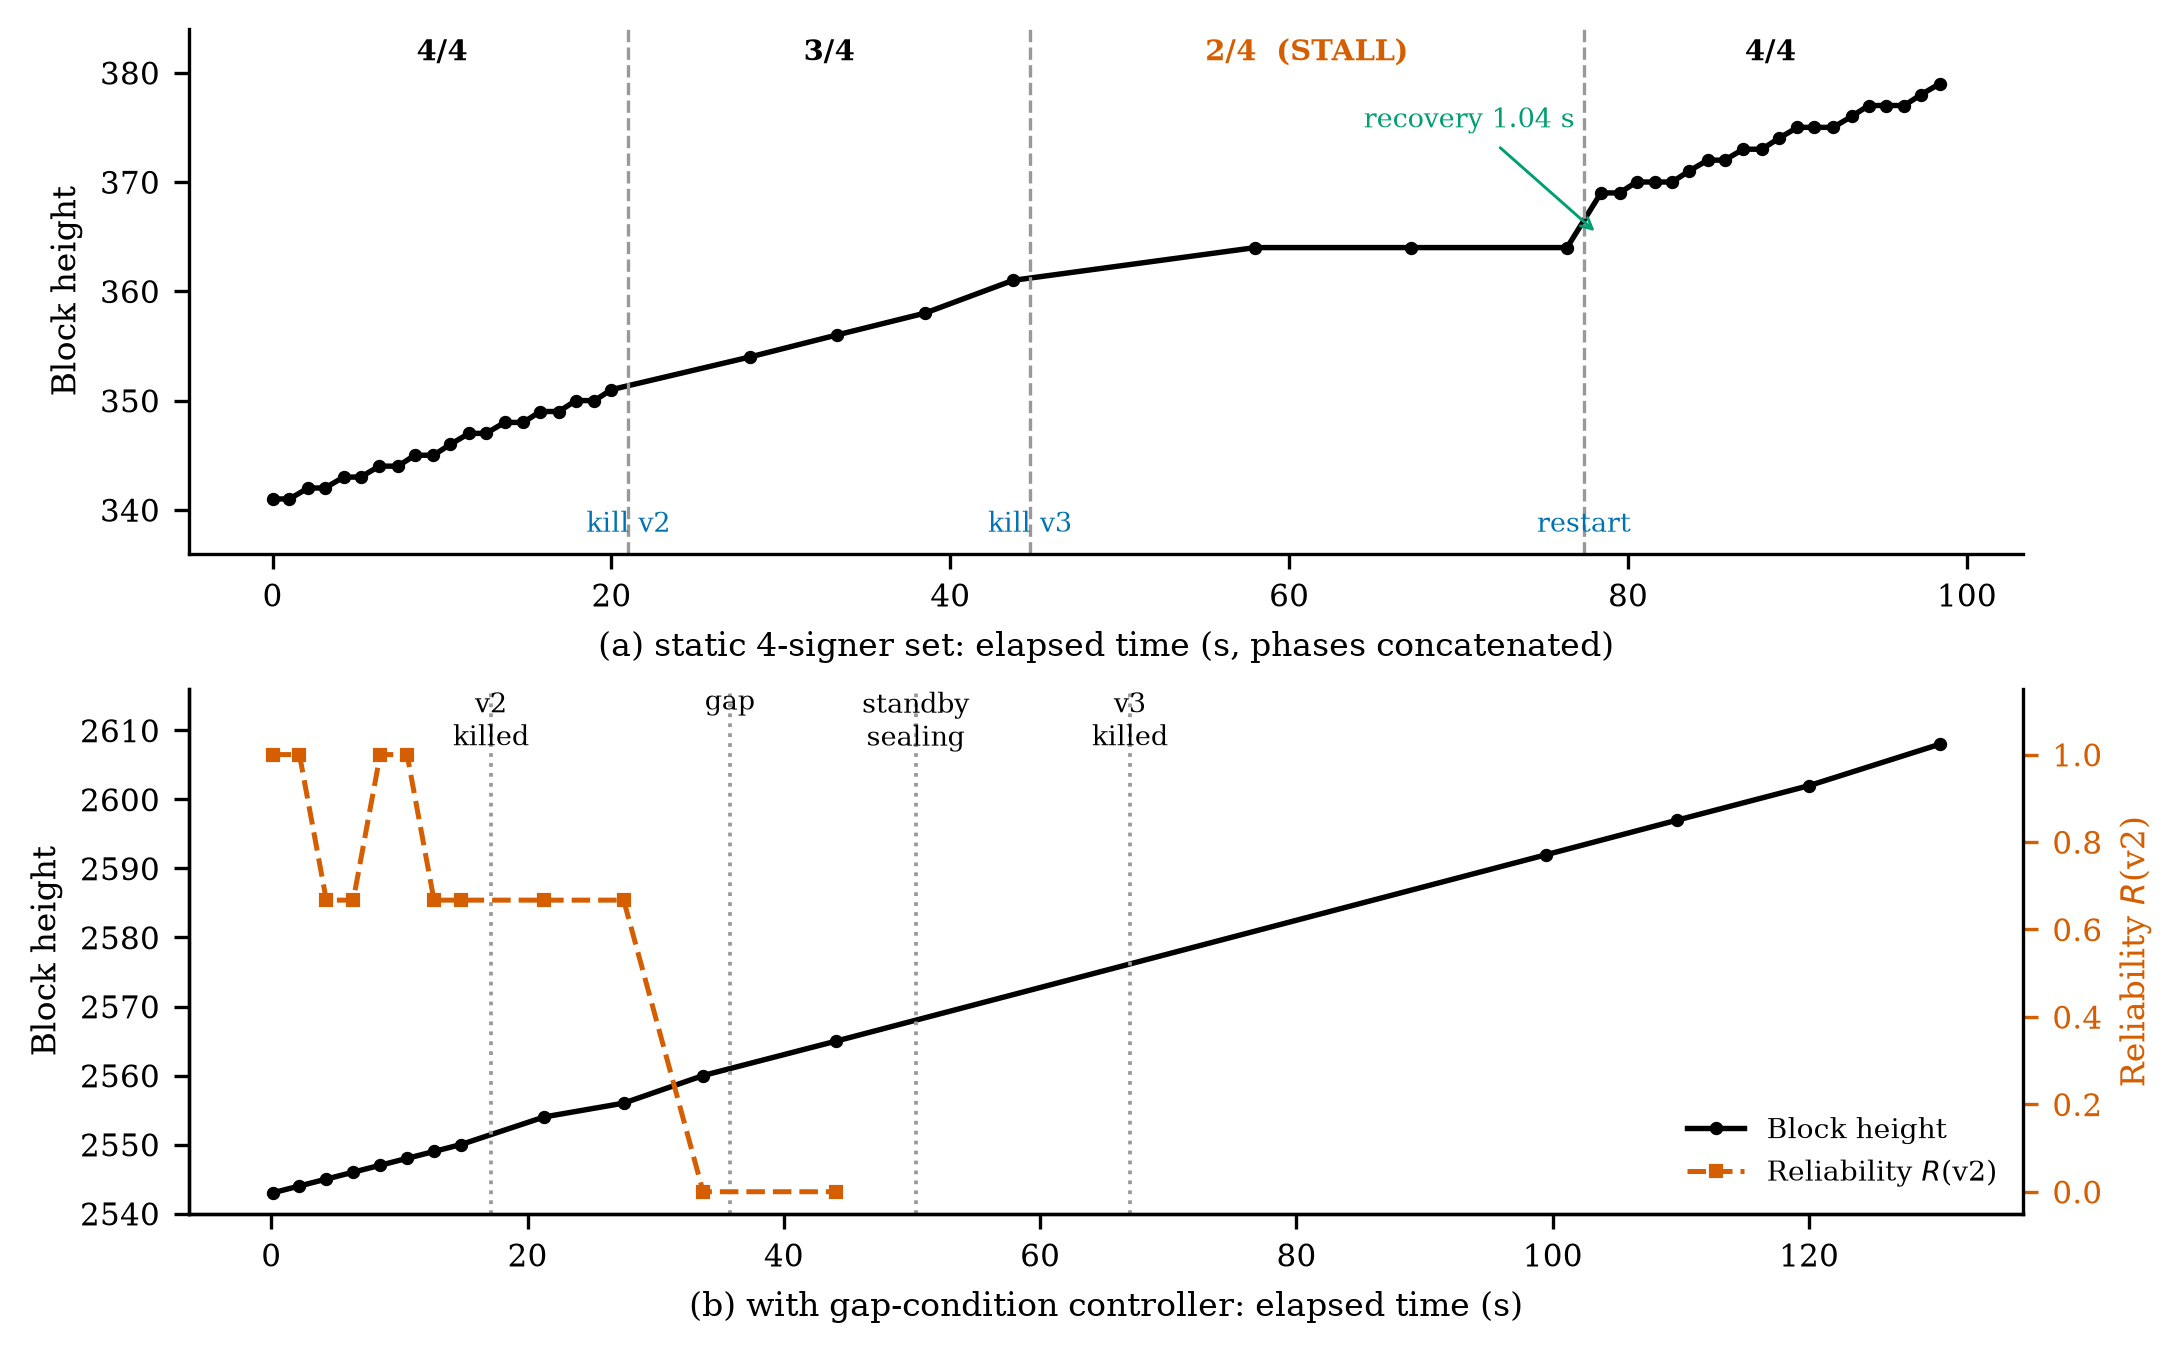
\includegraphics[width=1\columnwidth]{images/fig4_failure_timeline.png}
\caption{\textcolor{black}{Validator failure injection on a
four-signer Clique testnet. (a)~Static signer set: block
height over time across fault phases---single-signer fault
preserves liveness, loss of signing majority stalls the
chain, and signer restart recovers sealing in $1.04$~s.
(b)~With the gap-condition controller: after a signer fault
the controller detects the reliability gap ($18.6$~s) and
promotes a standby signer to sealing ($33.1$~s), so a
subsequent second fault does not stall the healed set.}}
\label{fig:failure}
\end{figure}
%%% ============================================================
%%% V-C  MQTT INGESTION THROUGHPUT  →  FIGURE
%%% ============================================================
\subsection{\textbf{IoT Ingestion Throughput}}
\label{sec:mqtt-results}

Fig.~\ref{fig:mqtt} shows per-message pipeline and
cumulative end-to-end (E2E) latency for 10~messages
(50~compounds each), comparing sequential and async
bridge modes.

\begin{figure}[!t]
\centering
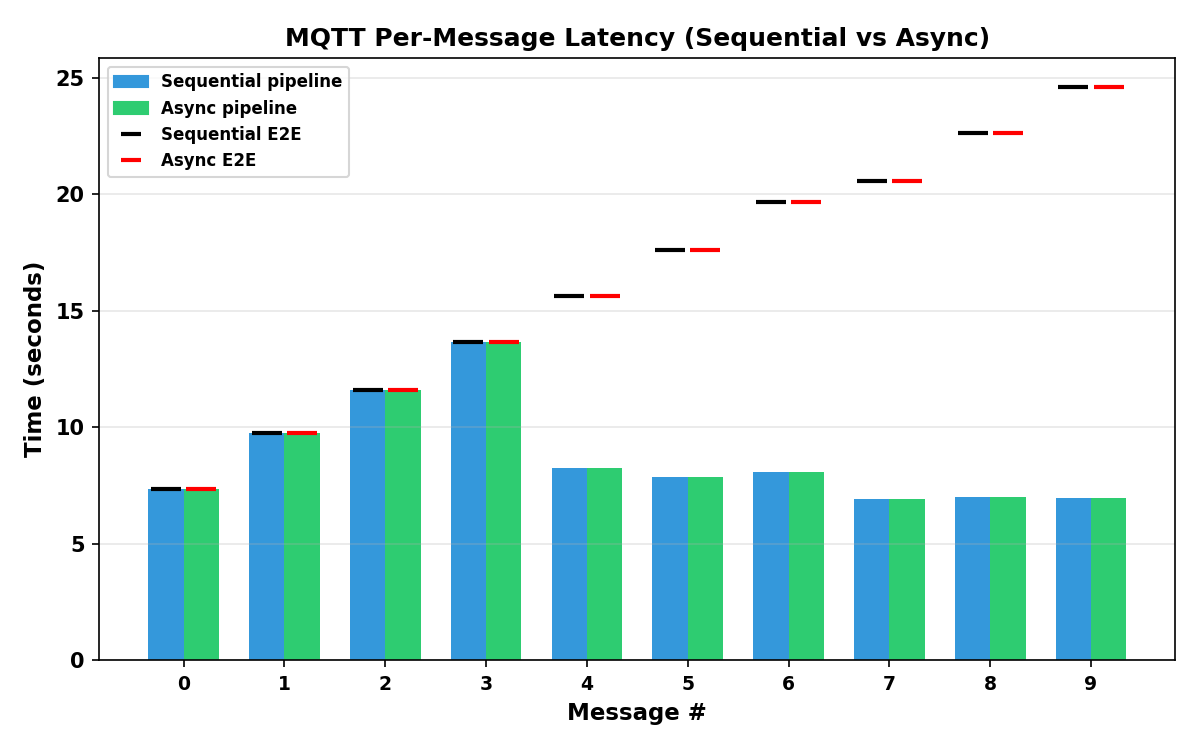
\includegraphics[width=\columnwidth]{images/fig_vd_mqtt_latency.png}
\caption{MQTT per-message pipeline (bars) and cumulative
E2E (horizontal lines) latency for sequential (blue/black)
and async (green/red) modes.
Async reduces median E2E latency by 17\% and achieves
100\%~blockchain commit success via thread-safe nonce
management (blocks~1{,}011{,}650--1{,}012{,}536).}
\label{fig:mqtt}
\end{figure}

The sequential bridge achieves 100\%~blockchain commit
success with 2{,}009~ms per-message pipeline latency
(median) and 19{,}706~ms median E2E latency.
The async bridge (4-worker \texttt{ThreadPoolExecutor}
with nonce manager) reduces median E2E latency to
16{,}315~ms ($-17\%$) and throughput from 18 to
20~compounds/s, while recovering 100\%~commit success
from the 80\%~success rate of the initial prototype
(which suffered concurrent nonce collisions).
The bottleneck in both modes is serialised blockchain
commits through the nonce manager; Merkle batch anchoring
(Section~\ref{sec:scalability-results}) is the
architectural path to eliminating this bottleneck.


%%% ============================================================
%%% V-D  BLOCKCHAIN SCALABILITY  →  FIGURE
%%% ============================================================
\subsection{\textbf{Blockchain Scalability and Merkle Efficiency}}
\label{sec:scalability-results}

Fig.~\ref{fig:scalability} compares per-record anchoring
latency for Strategy~A (individual commits) and
Strategy~B (Merkle batch) across three batch sizes on
real PureChain transactions.

\begin{figure}[!t]
\centering
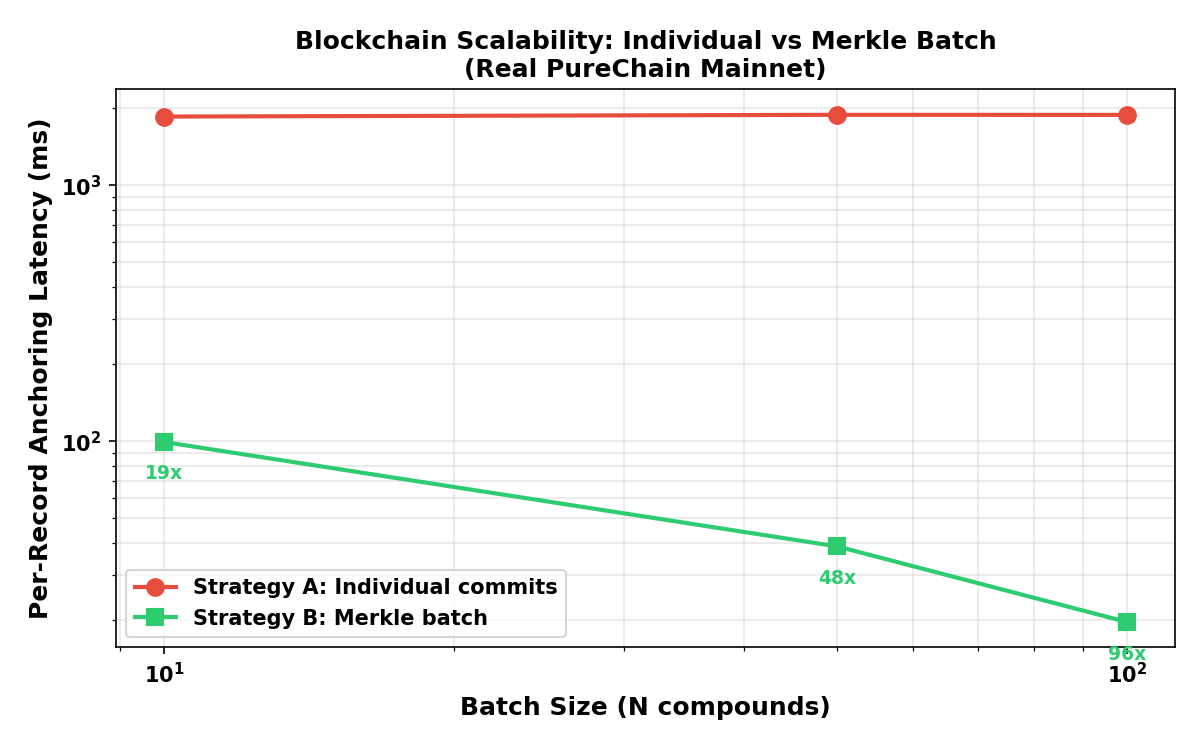
\includegraphics[width=\columnwidth]{images/fig_ve_scalability.png}
\caption{Per-record blockchain anchoring latency vs.\
batch size~$N$ (log--log scale). Strategy~A (red) is
constant at ${\sim}2$~s/record; Strategy~B (green) falls
as $1/N$, yielding 8.6$\times$, 48$\times$, and
94$\times$ speedup at $N{=}10$, 50, and 100 respectively.
Crossover $N^*{=}10$.}
\label{fig:scalability}
\end{figure}

Strategy~A per-record latency is constant at
${\sim}2{,}000$~ms, dominated by one PureChain round-trip
per transaction.
Strategy~B amortises one round-trip across $N$~records:
199~ms at $N{=}10$, 38.8~ms at $N{=}50$,
and 21.2~ms at $N{=}100$ (94$\times$ speedup),
while preserving full selective verifiability via Merkle
proof in $O(\log N)$ time.
The crossover $N^*{=}10$ is reached at the smallest
tested batch size, making Merkle batching the preferred
anchoring strategy for any IoT screening campaign.
Projecting to $N{=}10{,}000$ compounds: Strategy~A
requires ${\sim}5.5$~hours; Strategy~B requires
${\sim}2$~seconds.
\textcolor{black}{Both strategies are variants of the same
on-chain anchoring step; a fair comparison against
non-blockchain provenance mechanisms is given in
Section~\ref{sec:provenance-baselines}.}

\begin{figure}[!htbp]
\centering
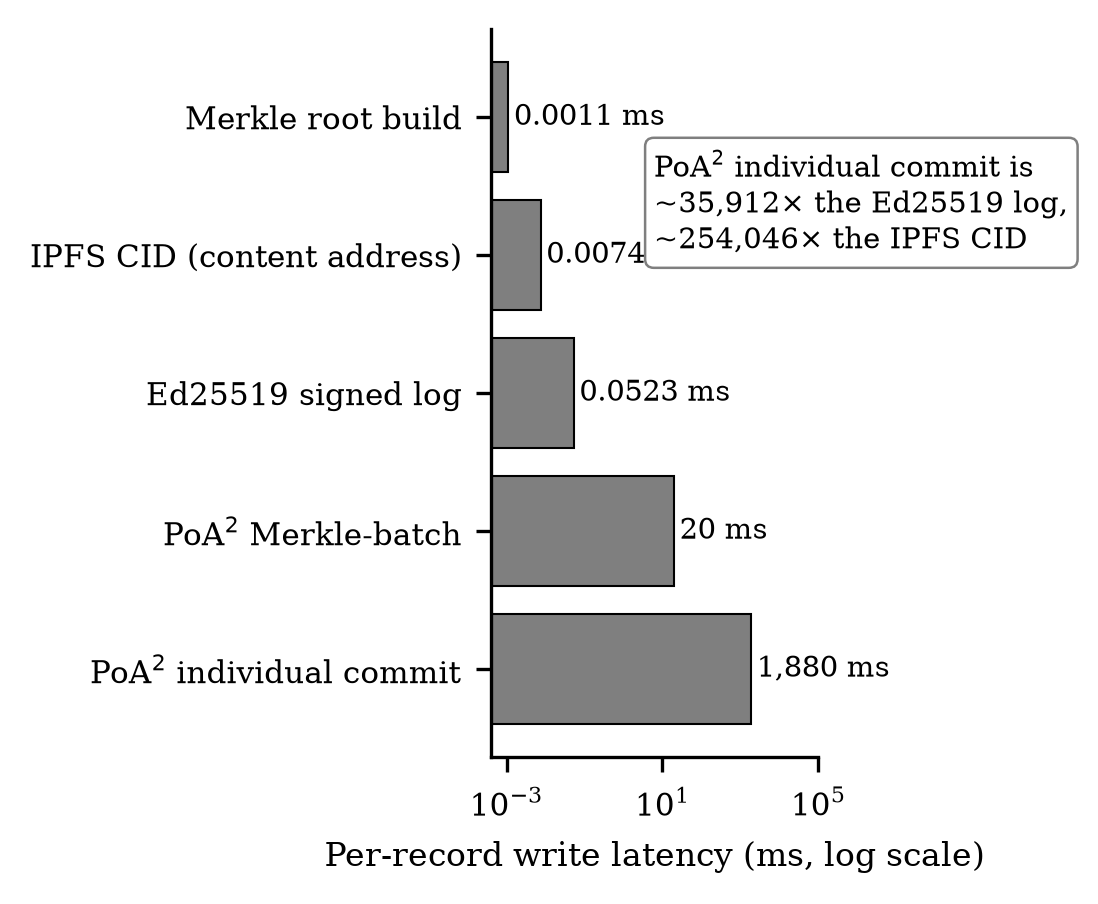
\includegraphics[width=\columnwidth]{images/fig3_provenance_cost.png}
\caption{\textcolor{black}{Per-record write latency of
provenance mechanisms (log scale): Merkle root build, IPFS CID,
Ed25519 signed log, and on-chain anchoring (Merkle-batched and
individual commit). Local mechanisms are microseconds; on-chain
anchoring incurs a consensus round-trip. The on-chain approach
is not competitive on cost; its advantage is the trust model
(Table~\ref{tab:trustmatrix}).}}
\label{fig:provcost}
\end{figure}

\textcolor{black}{\subsection{\textbf{ Comparison with Alternative Provenance Mechanisms}}
\label{sec:provenance-baselines}
The Merkle-batching result in Section~\ref{sec:scalability-results}
is an optimization within the on-chain anchoring step,
not a provenance baseline. To assess the on-chain approach
fairly, we compare it against two established alternatives that
provide tamper-evidence without a blockchain: an Ed25519 signed
append-only log (hash-chained entries, each signed) and
IPFS-style content addressing (a CIDv1 content hash over the
canonical payload). We compare on two axes---per-record cost and
trust model---in Fig.~\ref{fig:provcost} and
Table~\ref{tab:trustmatrix}.}

\begin{table}[!htbp]
\centering
\caption{\textcolor{black}{Provenance mechanisms compared on
trust properties and per-record write cost. The on-chain approach
loses on cost and wins only on the trust axis.}}
\label{tab:trustmatrix}
\scalebox{0.72}{
\textcolor{black}{%
\begin{tabular}{p{1.5cm}p{1.9cm}p{1.9cm}p{1.6cm}p{1.6cm}}
\toprule
Mechanism & Single point of compromise & Rewrite resistance & Public verification & Write cost (ms/rec) \\
\midrule
Ed25519 signed log & The private key & Key holder can re-sign history & Needs trusted public key & 0.0523 \\
\addlinespace
IPFS content addressing & The CID publisher & None alone (no ordering) & Needs trusted CID index & 0.0074 \\
\addlinespace
Merkle batch & The anchor & Needs external anchor & Needs the anchor & 0.0011 \\
\addlinespace
On-chain PoA$^2$ & None (distributed) & Requires signing-majority collusion & On-chain records & 1{,}880 (indiv.) / 20 (batch) \\
\bottomrule
\end{tabular}}}
\end{table}

\textcolor{black}{On cost, the on-chain approach is not competitive,
and we do not claim otherwise: a signed log is roughly four
orders of magnitude faster per record and content addressing
roughly five, since both are local operations while on-chain
anchoring incurs a consensus round-trip. On trust, the
distinction reverses. A signed log is only as trustworthy as
its single signing key: whoever holds the key can silently
re-sign an altered history. Content addressing detects
modification but imposes no ordering and no protection against a
publisher substituting the authoritative identifier. The
permissioned ledger removes the single-key assumption---rewriting
history requires collusion of a signing majority rather than
compromise of one party---and exposes the record for independent
verification. The on-chain approach is therefore the appropriate
choice only when the trust model forbids a single authoritative
key holder and requires independent verifiability; where a
trusted operator is acceptable, a signed log is the cheaper and
simpler option. This scoping is the honest basis for using a
ledger, replacing the earlier individual-versus-batch
comparison.}
%%% ============================================================
%%% V-E  ONNX DETERMINISM  →  TABLE
%%% ============================================================
\subsection{\textbf{Cross-Platform Determinism via ONNX}}
\label{sec:onnx-results}

Table~\ref{tab:onnx} reports on-chain ONNX model hashes,
bitwise determinism across 40~independent inference runs,
and sklearn-to-ONNX concordance for all 7~models.

\begin{table}[!t]
\centering
\caption{ONNX model export: on-chain SHA-256 hashes
(blocks~1{,}012{,}021--1{,}012{,}038), bitwise determinism
across 40~runs, and sklearn concordance.
R:~regression; C:~classification.}
\label{tab:onnx}
\scalebox{0.72}{
\begin{tabular}{llccc}
\toprule
\textbf{Model} & \textbf{SHA-256 (24 chars)}
  & \textbf{Block} & \textbf{Det.} & \textbf{Conc.} \\
\midrule
Scaler       & \texttt{66597669a2fa3f0c40ae783d}
  & 1{,}012{,}021 & \checkmark & \checkmark \\
R:SVR        & \texttt{884bb5709ca80c89812880b5}
  & 1{,}012{,}024 & \checkmark & \checkmark$^\dagger$ \\
R:RF         & \texttt{32dde6e15390fc572e81b293}
  & 1{,}012{,}027 & \checkmark & \checkmark \\
R:GB         & \texttt{20035ca63ca89ebd2dc52d7b}
  & 1{,}012{,}029 & \checkmark & \checkmark \\
C:SVC        & \texttt{287acaca13ad5815f8719d35}
  & 1{,}012{,}033 & \checkmark & \checkmark \\
C:RF         & \texttt{99be2e50f97b804fb58e42e7}
  & 1{,}012{,}036 & \checkmark & \checkmark \\
C:GB         & \texttt{2f59eaa7edf951c47555331b}
  & 1{,}012{,}038 & \checkmark & \checkmark \\
\midrule
\multicolumn{5}{l}{\footnotesize $^\dagger$ SVR:
  max\_diff~$= 2.12{\times}10^{-4}$ (float32/float64
  RBF kernel; $0.003\%$ of pIC$_{50}$ range).} \\
\multicolumn{5}{l}{\footnotesize Det.~= bitwise-identical
  across 40 runs (unique hash $= 1$).} \\
\multicolumn{5}{l}{\footnotesize Conc.~= concordant with
  sklearn within stated tolerance.}
\end{tabular}}
\end{table}

\textcolor{black}{Within a fixed configuration, all 7 models are
bitwise-deterministic across 40 independent runs and concordant with sklearn
outputs within characterised tolerances (Table~VIII). All ONNX model hashes
are anchored on-chain, enabling any edge node to verify it is running the
authorised model version by comparing its local ONNX binary hash against the
immutable on-chain record. The extent to which this determinism holds across
runtime versions, thread counts, and CPU architectures is characterized
below.}

\begin{figure*}[!htbp]
\centering
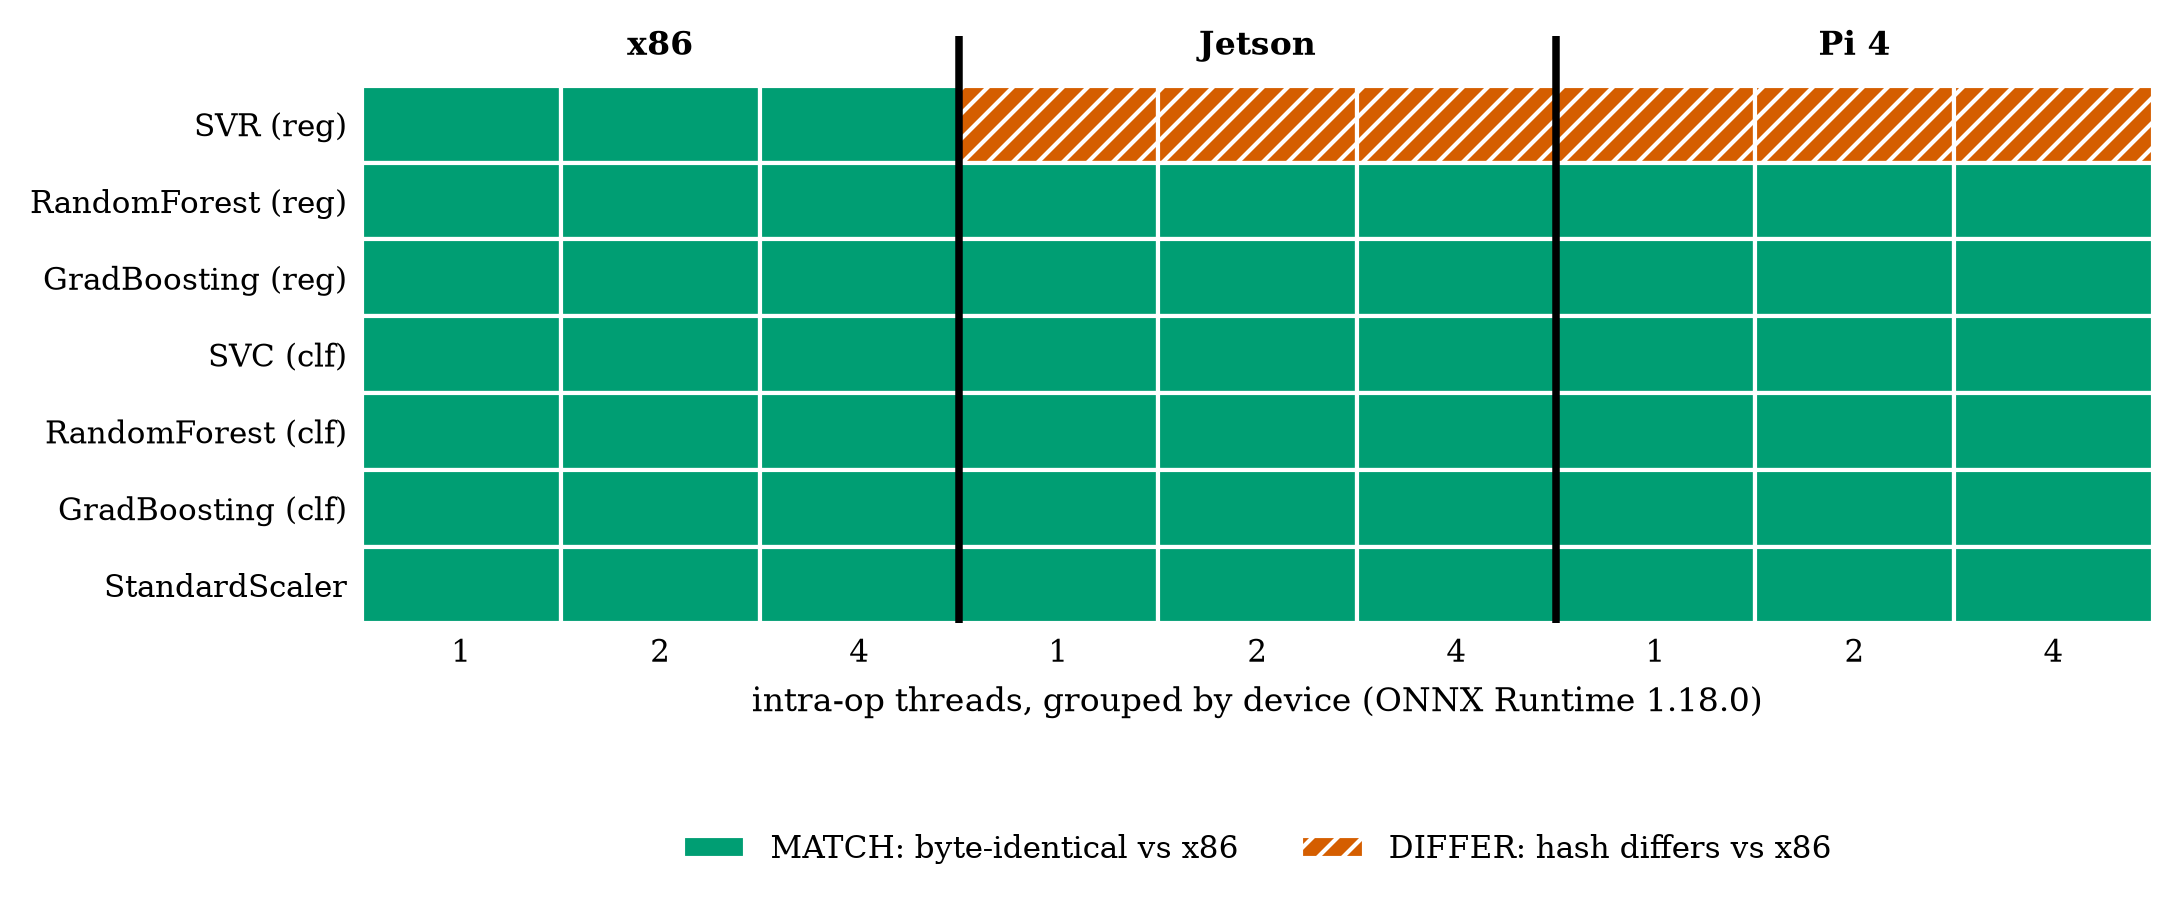
\includegraphics[width=0.95\textwidth]{images/fig1_cross_arch.png}
\caption{\textcolor{black}{Cross-architecture determinism
matrix: per-model SHA-256 agreement across x86\_64, Jetson
Orin Nano (aarch64), and Raspberry Pi~4 (aarch64) at intra-op
thread counts $\{1,2,4\}$. Green: byte-identical to the x86
reference; hatched: digest differs. Six of seven models are
byte-identical across all three architectures; only the
RBF-kernel SVR diverges. The pattern is identical across ONNX
Runtime 1.17--1.22 (one representative version shown; full
matrix in the repository).}}
\label{fig:crossarch}
\end{figure*}

\textcolor{black}{To test the cross-platform claim directly, we
ran an identical determinism harness across ONNX Runtime
versions 1.17--1.22, intra-op thread counts $\{1,2,4\}$, both
float32 and float64 export paths, and three real CPU
architectures: x86\_64, the Jetson Orin Nano (aarch64), and
the Raspberry Pi~4 (aarch64). For each configuration the
harness executes 40 inference runs on a fixed seeded input
and compares SHA-256 digests. Fig.~\ref{fig:crossarch}
summarizes the cross-architecture result and
Table~\ref{tab:determinism-detail} the per-model detail.}

\begin{table}[!htbp]
\centering
\caption{\textcolor{black}{Per-model determinism
characterization: within-configuration (40 runs), across
intra-op thread counts, across ONNX Runtime 1.17--1.22, and
dtype residual versus the sklearn float64 reference.}}
\label{tab:determinism-detail}
\scalebox{0.78}{
\textcolor{black}{%
\begin{tabular}{p{2.5cm} p{1.5cm} p{1.5cm} p{1.5cm} p{2cm}}
\toprule
Model & Within-config & Cross-thread & Cross-ORT & dtype residual \\
      & (40 runs)     & \{1,2,4\}    & (1.17--1.22) & (vs sklearn) \\
\midrule
SVR (reg)          & identical & stable & stable & f32 $1.25{\times}10^{-4}$; f64 n/a$^\dagger$ \\
RandomForest (reg) & identical & varies & stable & f64 n/a$^\dagger$ \\
GradBoosting (reg)  & identical & varies & stable & f64 n/a$^\dagger$ \\
SVC (clf)          & identical & stable & stable & -- \\
RandomForest (clf) & identical & stable & stable & -- \\
GradBoosting (clf)  & identical & stable & stable & -- \\
StandardScaler     & identical & stable & stable & f32 $1.65{\times}10^{-5}$; f64 exact (0) \\
\bottomrule
\end{tabular}}}
\\[2pt]
{\footnotesize \textcolor{black}{$^\dagger$ ONNX Runtime has no
float64 \texttt{SVMRegressor} kernel (\texttt{NOT\_IMPLEMENTED});
tree float32/float64 re-export failed under the pinned
\texttt{onnx}~1.17 toolchain, so tree determinism is
characterized via the thread axis.}}
\end{table}

\textcolor{black}{Three findings result. First, within a fixed
thread count every model is bitwise-identical across all 40
runs and across ORT 1.17--1.22, and remains identical across
the NumPy 1.26$\rightarrow$2.5 boundary---stability stronger
than a single-runtime guarantee. Second, bitwise determinism
does \emph{not} hold across differing intra-op thread counts
for the tree-ensemble regressors (random forest and gradient
boosting), whose threaded reduction order changes the output
bytes; the scaler, SVR, and all classifiers are thread-stable.
Third, across the three architectures at a fixed thread count,
six of seven models are byte-identical; the sole exception is
the RBF-kernel SVR, which differs between x86\_64 and aarch64
because ONNX Runtime provides no double-precision SVR kernel
and its float32 kernel is architecture-sensitive. The residual
is $\sim$$10^{-4}$ in pIC$_{50}$, far below the $\sim$0.7 RMSE
of the task, so it is scientifically negligible while remaining
cryptographically visible.}

\textcolor{black}{Accordingly, PureProtX pins the intra-op thread
count alongside the ORT version and model-artifact hash in the
on-chain configuration record. Under this pinning, re-execution
is byte-identical across all three heterogeneous devices for
the thread-stable models; the SVR carries a per-architecture
digest, which the anchored configuration makes explicit rather
than silently violating.}


%%% ============================================================
%%% V-F  TAMPER DETECTION  →  FIGURE
%%% ============================================================
\subsection{\textbf{Tamper Detection}}
\label{sec:tamper-results}

Fig.~\ref{fig:tamper} demonstrates the framework's
tamper-evidence property at single-field granularity.

\begin{figure}[!htbp]
\centering
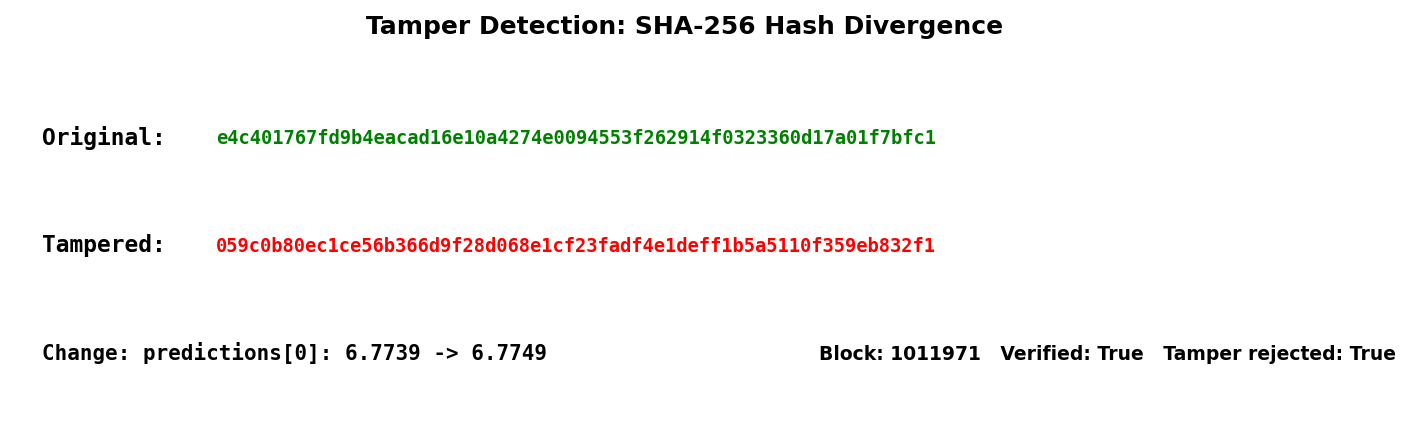
\includegraphics[width=\columnwidth]{images/fig_vg_tamper.png}
\caption{SHA-256 hash divergence under a $+0.001$ change
in one pIC$_{50}$ prediction (6.7739~$\to$~6.7749).
The original (\texttt{e4c401...}) and tampered
(\texttt{059c0b...}) digests are completely different;
the on-chain record at block~1{,}011{,}971 verifies
the original and rejects the tampered result.}
\label{fig:tamper}
\end{figure}

Modifying a single pIC$_{50}$ prediction by $+0.001$
produces a completely different 64-character SHA-256
digest, which immediately diverges from the immutable
on-chain record (block~1{,}011{,}971).
This confirms that canonical JSON serialisation
propagates even sub-unit numerical perturbations into
a detectable hash difference, providing cryptographic
proof of result integrity at the level of individual
predicted values --- a property directly relevant to
regulatory-grade computational evidence requirements.

\begin{figure*}[!htbp]
\centering
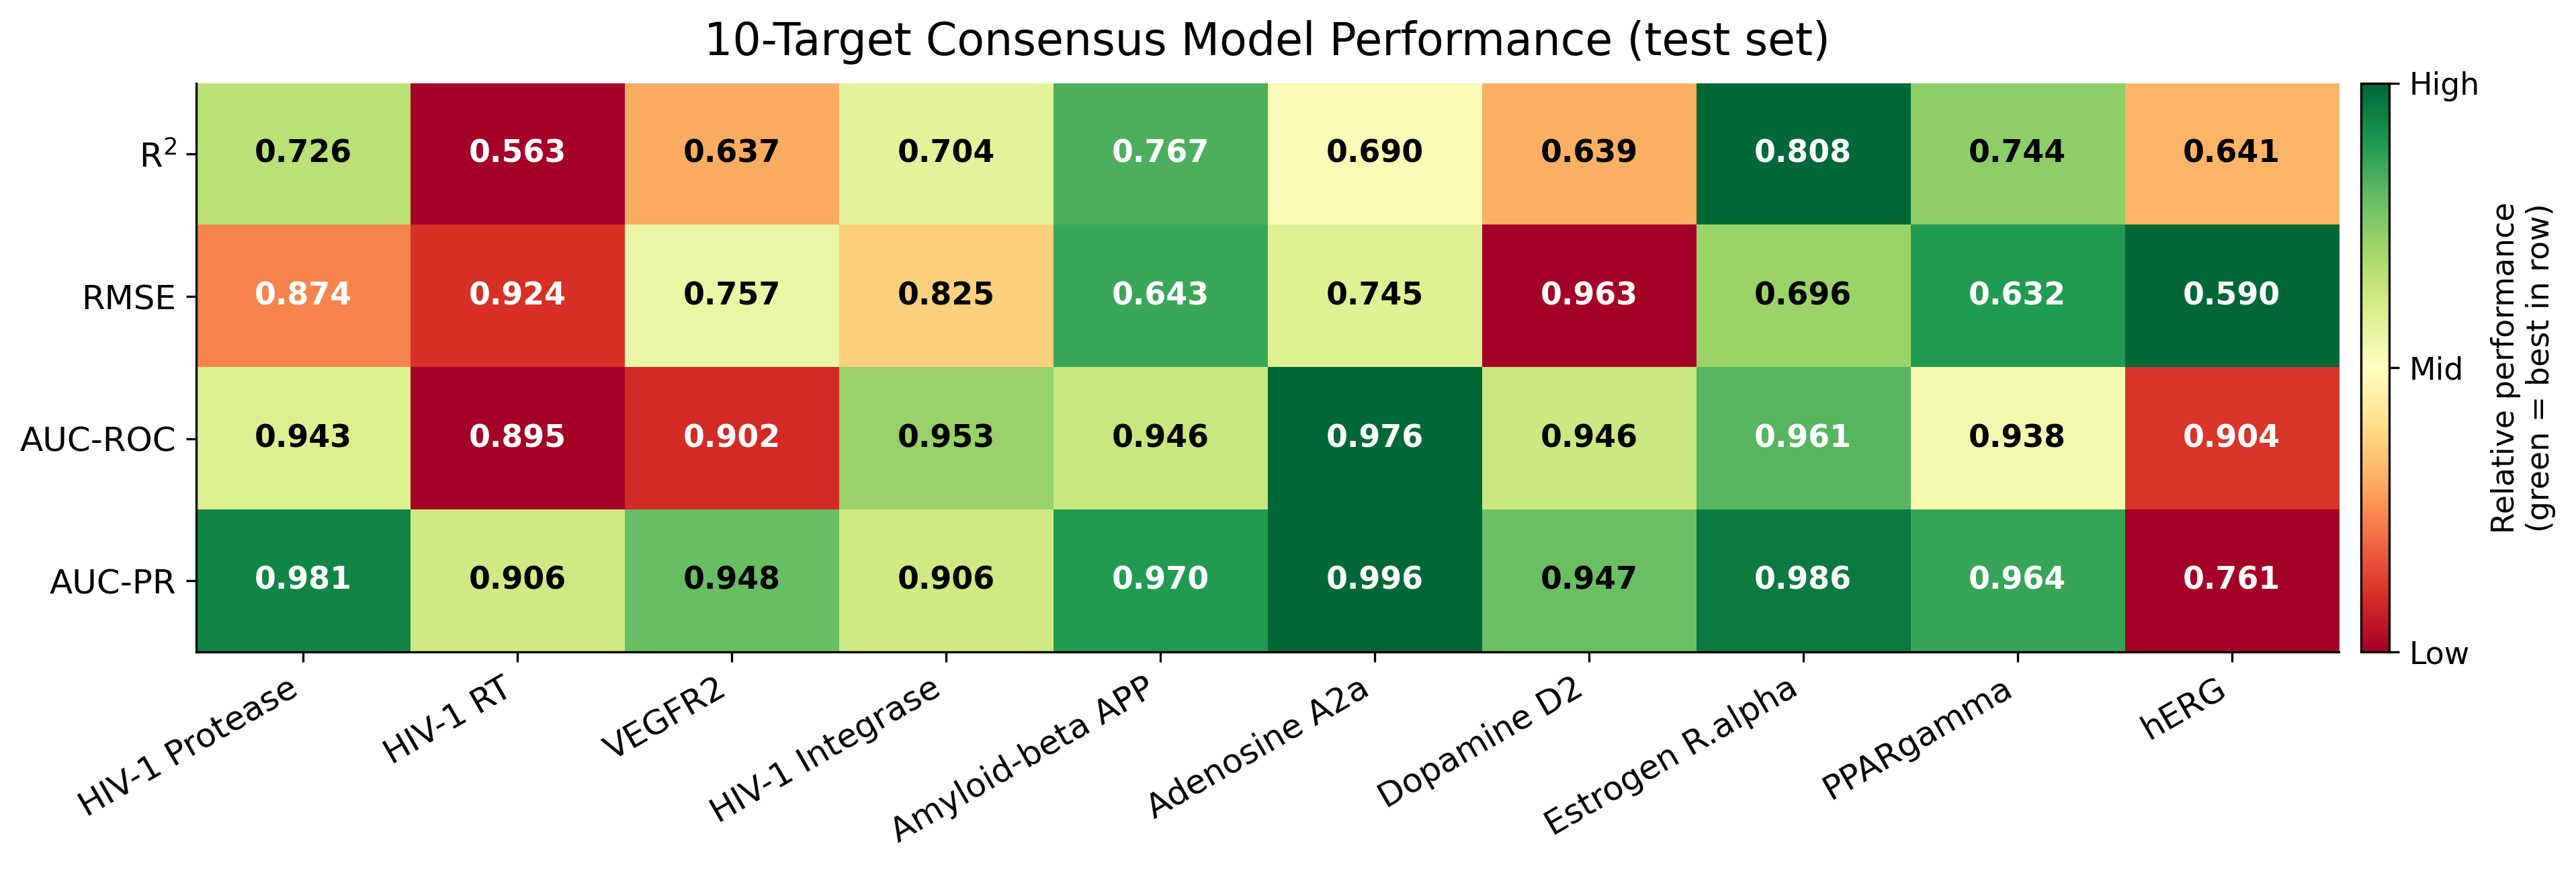
\includegraphics[width=0.95\textwidth]{images/fig_C1_performance_heatmap.png}
\caption{Consensus model performance across 10~targets
(test set). Colour intensity indicates relative performance
within each metric row (green~$=$~best). Mean
$R^2{=}0.693$, RMSE~$= 0.763$,
AUC-ROC~$= 0.937$, AUC-PR~$= 0.946$.}
\label{fig:heatmap}
\end{figure*}

% --- Alpha figure ---
\begin{figure*}[!htbp]
\centering
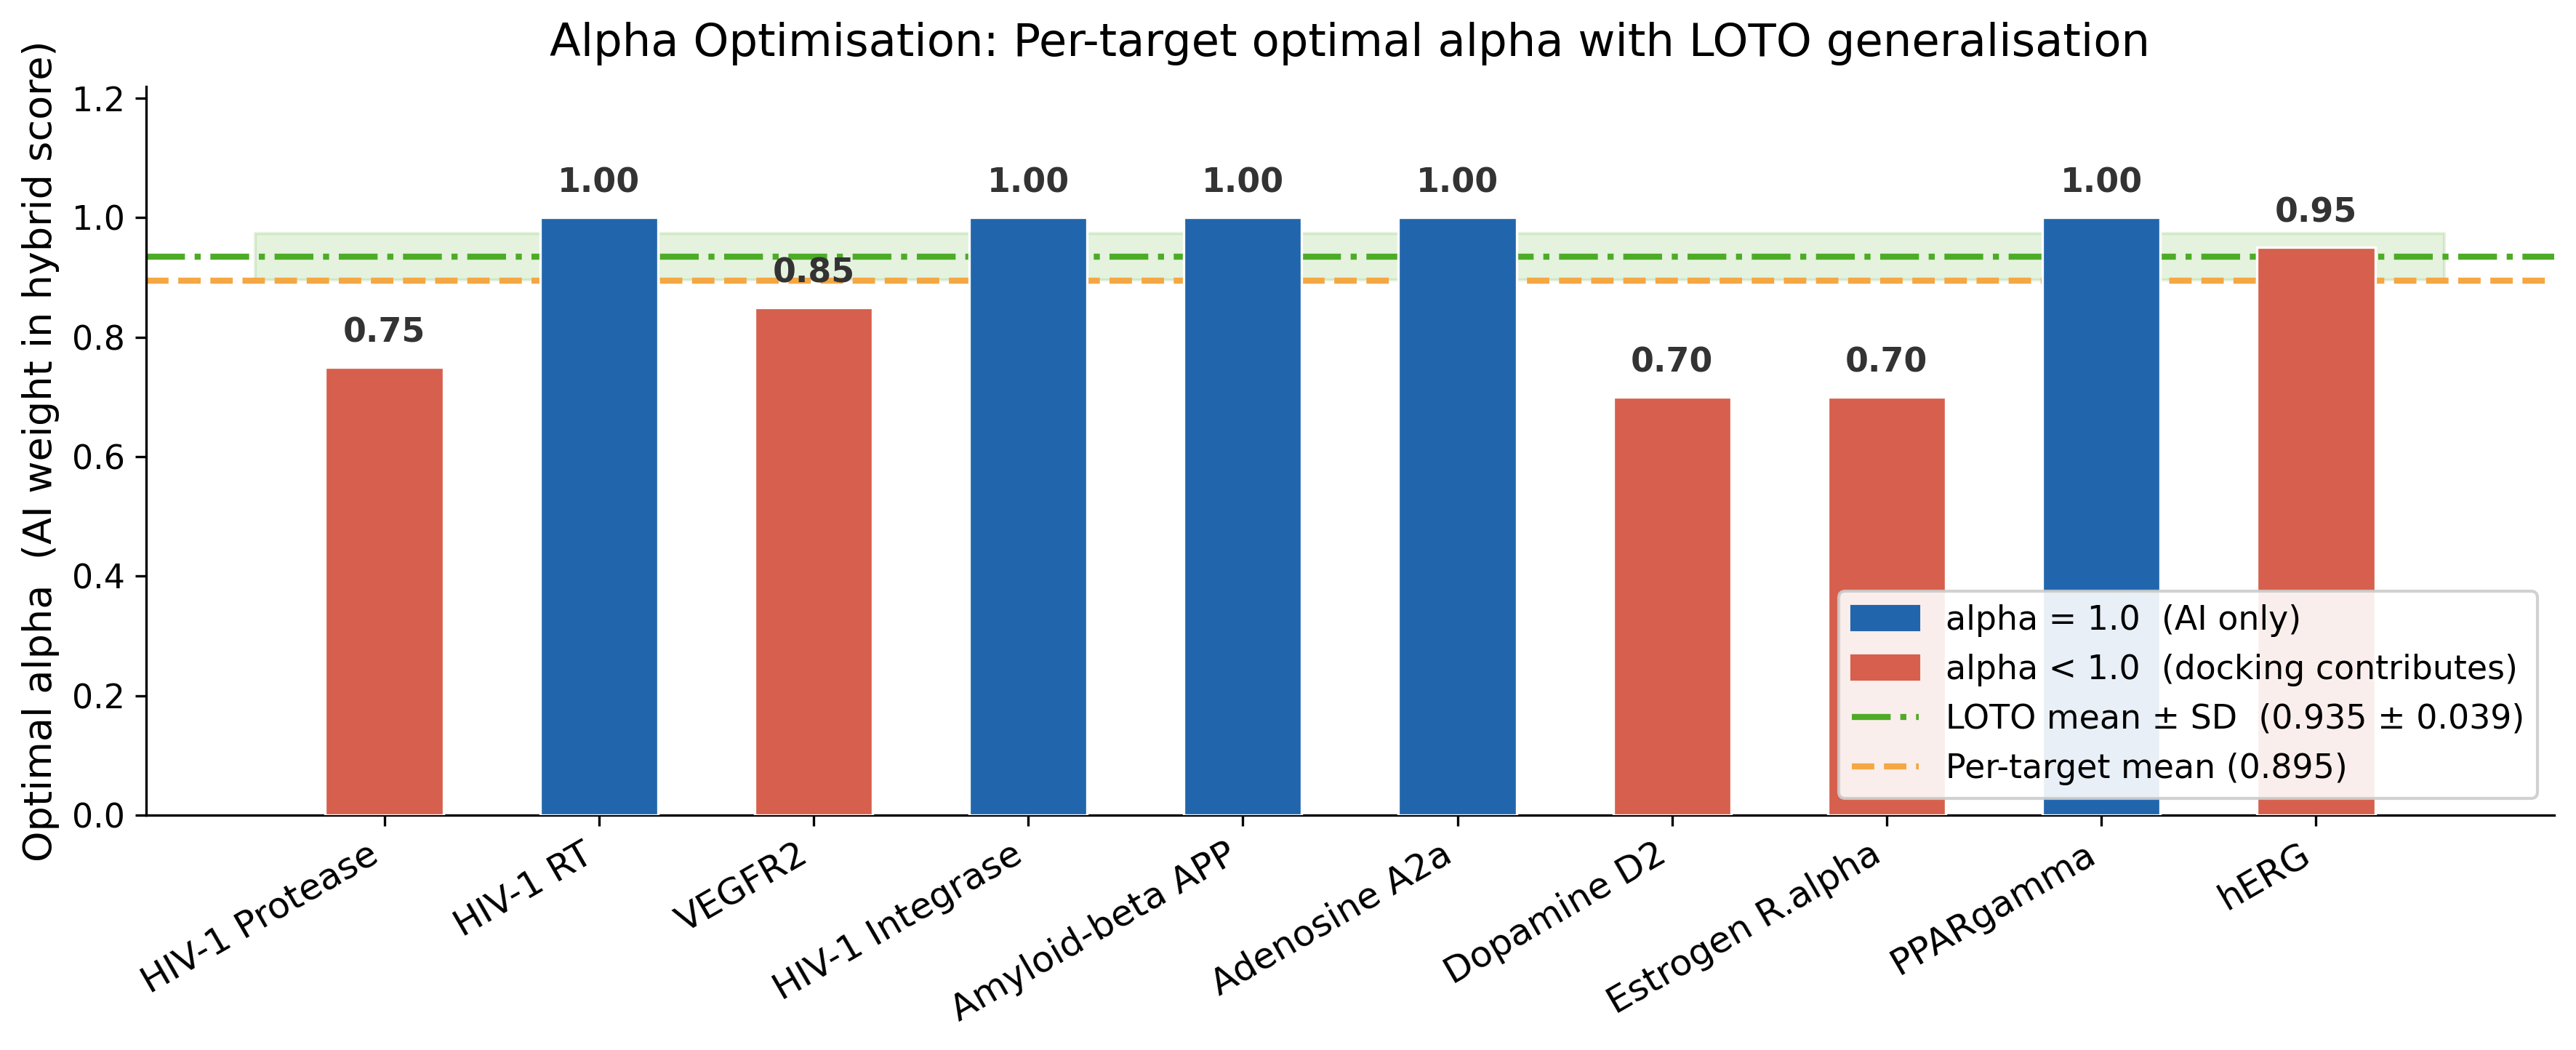
\includegraphics[width=\linewidth]{images/fig_D1_alpha_optimization.png}
\caption{Per-target optimal $\alpha$ (AI weight in hybrid score). Blue bars indicate targets where $\alpha = 1.0$ (AI only); red bars indicate targets where docking contributes ($\alpha < 1.0$). Dashed lines show the per-target mean ($0.895$) and LOTO cross-validated mean ($0.935 \pm 0.039$).}
\label{fig:alpha}
\end{figure*}
%%% ============================================================
%%% V-G  BLOCKCHAIN OVERHEAD  →  TABLE
%%% ============================================================
\subsection{\textbf{Blockchain Anchoring Overhead}}
\label{sec:overhead-results}

Table~\ref{tab:overhead} quantifies the exact provenance
cost across two targets representing the extremes of
model complexity, plus the Merkle-batched regime.

\begin{table}[!t]
\centering
\caption{Blockchain anchoring overhead at $N{=}1{,}000$
compounds (5~repeated runs, median). With Merkle batching
at $N{=}100$: $<0.01\%$ per record.}
\label{tab:overhead}
\scalebox{0.82}{
\begin{tabular}{lrrrr}
\toprule
\textbf{Target} & \textbf{Pipeline (s)}
  & \textbf{+Chain (s)} & \textbf{Overhead (s)}
  & \textbf{Overhead (\%)} \\
\midrule
CHEMBL243 & 3.31  & 4.67  & 1.36 & 41.1 \\
CHEMBL240 & 14.34 & 15.03 & 0.70 &  4.9 \\
\midrule
\multicolumn{5}{l}{\footnotesize Merkle batch
  $N{=}100$: 21~ms/record ($<0.01\%$).}
\end{tabular}}
\end{table}

The PureChain commit adds a fixed ${\sim}1.4$~s per batch
(PoA$^2$ consensus round-trip), representing 41.1\%
overhead for CHEMBL243 (3.31~s inference) but only 4.9\%
for hERG (14.34~s inference), scaling inversely with
inference complexity.
These three figures define the deployment operating
envelope: 41.1\% for small single-record commits;
4.9\% for large single-record commits; $<0.01\%$
per record with Merkle batching at $N{\geq}100$.
Provenance overhead is therefore negligible at any
realistic IoT screening campaign scale.


%%% ============================================================
%%% V-H  CONSENSUS AI PERFORMANCE  →  FIGURE
%%% ============================================================
\subsection{\textbf{Consensus AI Performance}}
\label{sec:ai-results}

Fig.~\ref{fig:heatmap} summarises test-set performance of
the consensus AI module across all 10~targets, validating
that the IoT infrastructure sustains a non-trivial
scientific workload.



The regression ensemble (SVR, RF, GB, MLP) achieved mean
$R^2{=}0.693$ and RMSE~$=0.763$, with per-target $R^2$
ranging from 0.563 (HIV-1~RT, most heterogeneous dataset)
to 0.808 (ER$\alpha$).
The classification ensemble (SVC, RF, GB) with isotonic
calibration achieved mean AUC-ROC~$=0.937$ and
AUC-PR~$=0.946$, with mean BSS~$=0.577{\pm}0.037$
confirming well-calibrated probabilities substantially
above the na\"ive prevalence baseline.
Grid-searched hyperparameters improved mean $R^2$ by +0.035 and RMSE by
$-0.037$ relative to defaults. \textcolor{black}{All pipeline components are
bitwise-reproducible within a pinned runtime configuration; the extent of
this determinism across runtime versions, thread counts, and CPU
architectures is characterized in Section~V-F.}


%%% ============================================================
%%% V-I  HYBRID CONSENSUS  →  TABLE
%%% ============================================================
\subsection{\textbf{Hybrid AI--Docking Consensus Evaluation}}
\label{sec:hybrid-results}

Table~\ref{tab:enrichment} presents early-recognition
metrics for all 10~targets across regression,
classification, and hybrid scoring modes, with per-target
optimal $\alpha$ from validation-set grid search.
Per-target $\alpha$ values are additionally summarised
in Fig.~\ref{fig:alpha} in the supplementary material.

\begin{table}[!htbp]
\centering
\caption{Exhaustiveness sensitivity analysis. Spearman rank correlation ($\rho$) between per-molecule Vina scores at $e{=}1$ and $e{=}4$ on the test set.}
\label{tab:supp-exhaust}
\scalebox{0.78}{
\begin{tabular}{p{2.5cm} p{2.5cm} p{1.5cm} p{2cm}}
\toprule
\textbf{Target} & \textbf{Family} & \textbf{$\rho$ (test)} & \textbf{Interpretation} \\
\midrule
HIV-1 Protease     & Viral protease   & 0.954 & Stable \\
hERG               & Ion channel      & 0.959 & Stable \\
Dopamine D$_2$     & GPCR             & 0.942 & Stable \\
APP                & Membrane protein & 0.880 & Good \\
HIV-1 Integrase    & Viral integrase  & 0.822 & Good \\
ER$\alpha$         & Nuclear receptor & 0.821 & Good \\
VEGFR2             & Kinase           & 0.758 & Moderate \\
HIV-1 RT           & Viral polymerase & 0.688 & Moderate \\
Adenosine A$_{2a}$ & GPCR             & 0.644 & Moderate \\
PPAR$\gamma$       & Nuclear receptor & 0.622 & Weakest \\
\midrule
\textbf{Mean}      &                  & \textbf{0.809} & \\
\bottomrule
\end{tabular}}
\end{table}

% --- Enrichment table ---
\begin{table*}[!t]
\centering
\caption{Early-recognition metrics on ChEMBL test sets. EF = enrichment factor; BEDROC computed at $\alpha{=}20$. Hybrid $\alpha$ values are per-target optima from validation-set grid search.}
\label{tab:enrichment}
\scalebox{0.72}{
\begin{tabular}{p{3cm} p{3cm}  p{3cm} p{3cm} p{3cm}  p{3cm} p{3cm}}
\toprule
\textbf{Target} & \textbf{Method} & \textbf{EF@1\%} & \textbf{EF@5\%} & \textbf{EF@10\%} & \textbf{BEDROC} & \textbf{AUC-ROC} \\
\midrule
HIV-1 Protease & Regression & 1.29 & 1.29 & 1.29 & 0.882 & 0.940 \\
 & Classification & 1.29 & 1.29 & 1.29 & 0.877 & 0.943 \\
 & Hybrid ($\alpha{=}0.75$) & 1.29 & 1.29 & 1.29 & 0.882 & 0.943 \\
\midrule
HIV-1 RT & Regression & 1.83 & 1.76 & 1.74 & 0.887 & 0.884 \\
 & Classification & 1.83 & 1.79 & 1.77 & 0.916 & 0.895 \\
 & Hybrid ($\alpha{=}1.00$) & 1.83 & 1.76 & 1.74 & 0.887 & 0.884 \\
\midrule
VEGFR2 & Regression & 1.52 & 1.52 & 1.51 & 0.966 & 0.890 \\
 & Classification & 1.47 & 1.51 & 1.51 & 0.952 & 0.902 \\
 & Hybrid ($\alpha{=}0.85$) & 1.52 & 1.51 & 1.50 & 0.958 & 0.883 \\
\midrule
HIV-1 Integrase & Regression & 3.43 & 3.34 & 3.27 & 0.922 & 0.935 \\
 & Classification & 3.43 & 3.38 & 3.36 & 0.948 & 0.953 \\
 & Hybrid ($\alpha{=}1.00$) & 3.43 & 3.34 & 3.27 & 0.922 & 0.935 \\
\midrule
APP & Regression & 1.44 & 1.44 & 1.44 & 0.742 & 0.944 \\
 & Classification & 1.44 & 1.44 & 1.44 & 0.720 & 0.946 \\
 & Hybrid ($\alpha{=}1.00$) & 1.44 & 1.44 & 1.44 & 0.742 & 0.944 \\
\midrule
Adenosine A$_{2a}$ & Regression & 1.15 & 1.15 & 1.15 & 0.735 & 0.924 \\
 & Classification & 1.15 & 1.15 & 1.15 & 0.736 & 0.976 \\
 & Hybrid ($\alpha{=}1.00$) & 1.15 & 1.15 & 1.15 & 0.735 & 0.924 \\
\midrule
Dopamine D$_2$ & Regression & 1.95 & 1.95 & 1.89 & 0.848 & 0.943 \\
 & Classification & 1.95 & 1.95 & 1.89 & 0.851 & 0.946 \\
 & Hybrid ($\alpha{=}0.70$) & 1.95 & 1.83 & 1.89 & 0.792 & 0.904 \\
\midrule
ER$\alpha$ & Regression & 1.30 & 1.30 & 1.29 & 0.909 & 0.957 \\
 & Classification & 1.30 & 1.27 & 1.29 & 0.863 & 0.961 \\
 & Hybrid ($\alpha{=}0.70$) & 1.30 & 1.30 & 1.30 & 0.917 & 0.929 \\
\midrule
PPAR$\gamma$ & Regression & 1.50 & 1.50 & 1.50 & 0.959 & 0.922 \\
 & Classification & 1.43 & 1.49 & 1.50 & 0.936 & 0.938 \\
 & Hybrid ($\alpha{=}1.00$) & 1.50 & 1.50 & 1.50 & 0.959 & 0.922 \\
\midrule
hERG & Regression & 4.75 & 4.84 & 4.79 & 0.804 & 0.912 \\
 & Classification & 5.57 & 5.11 & 4.77 & 0.833 & 0.904 \\
 & Hybrid ($\alpha{=}0.95$) & 4.75 & 4.91 & 4.79 & 0.805 & 0.913 \\
\bottomrule
\end{tabular}}
\end{table*}



EF@1\% ranges from 1.15 (Adenosine~A$_{2a}$) to 5.57
(hERG, classification), with BEDROC spanning 0.720--0.966.
Five targets converge to $\alpha{=}1.0$, indicating
AutoDock Vina provides no enrichment benefit; the
remaining five ($\alpha{<}1.0$) receive genuine
complementary signal from structure-based docking.
A Wilcoxon signed-rank test on the 5~non-tied pairs
yields $p{=}1.000$ (statistic~$=7.0$): the hybrid does
not significantly outperform AI-only on ChEMBL data.
The contribution is a systematic characterisation of
\emph{when} docking adds value --- for rigid pockets
where Vina rankings are reproducible
($\rho{\geq}0.82$, Table~\ref{tab:supp-exhaust}) ---
rather than a claim of universal superiority.
The LOTO $\alpha{=}0.935{\pm}0.039$ provides a principled
deployment default for novel targets.


%%% ============================================================
%%% V-J  SCAFFOLD DIVERSITY  →  FIGURE
%%% ============================================================
\subsection{\textbf{Scaffold Diversity}}
\label{sec:scaffold-results}

Fig.~\ref{fig:scaffold} shows Bemis--Murcko novel scaffold
fraction in the top-10\% of predictions for the
5~targets where $\alpha{<}1.0$.

\begin{figure}[!htbp]
\centering
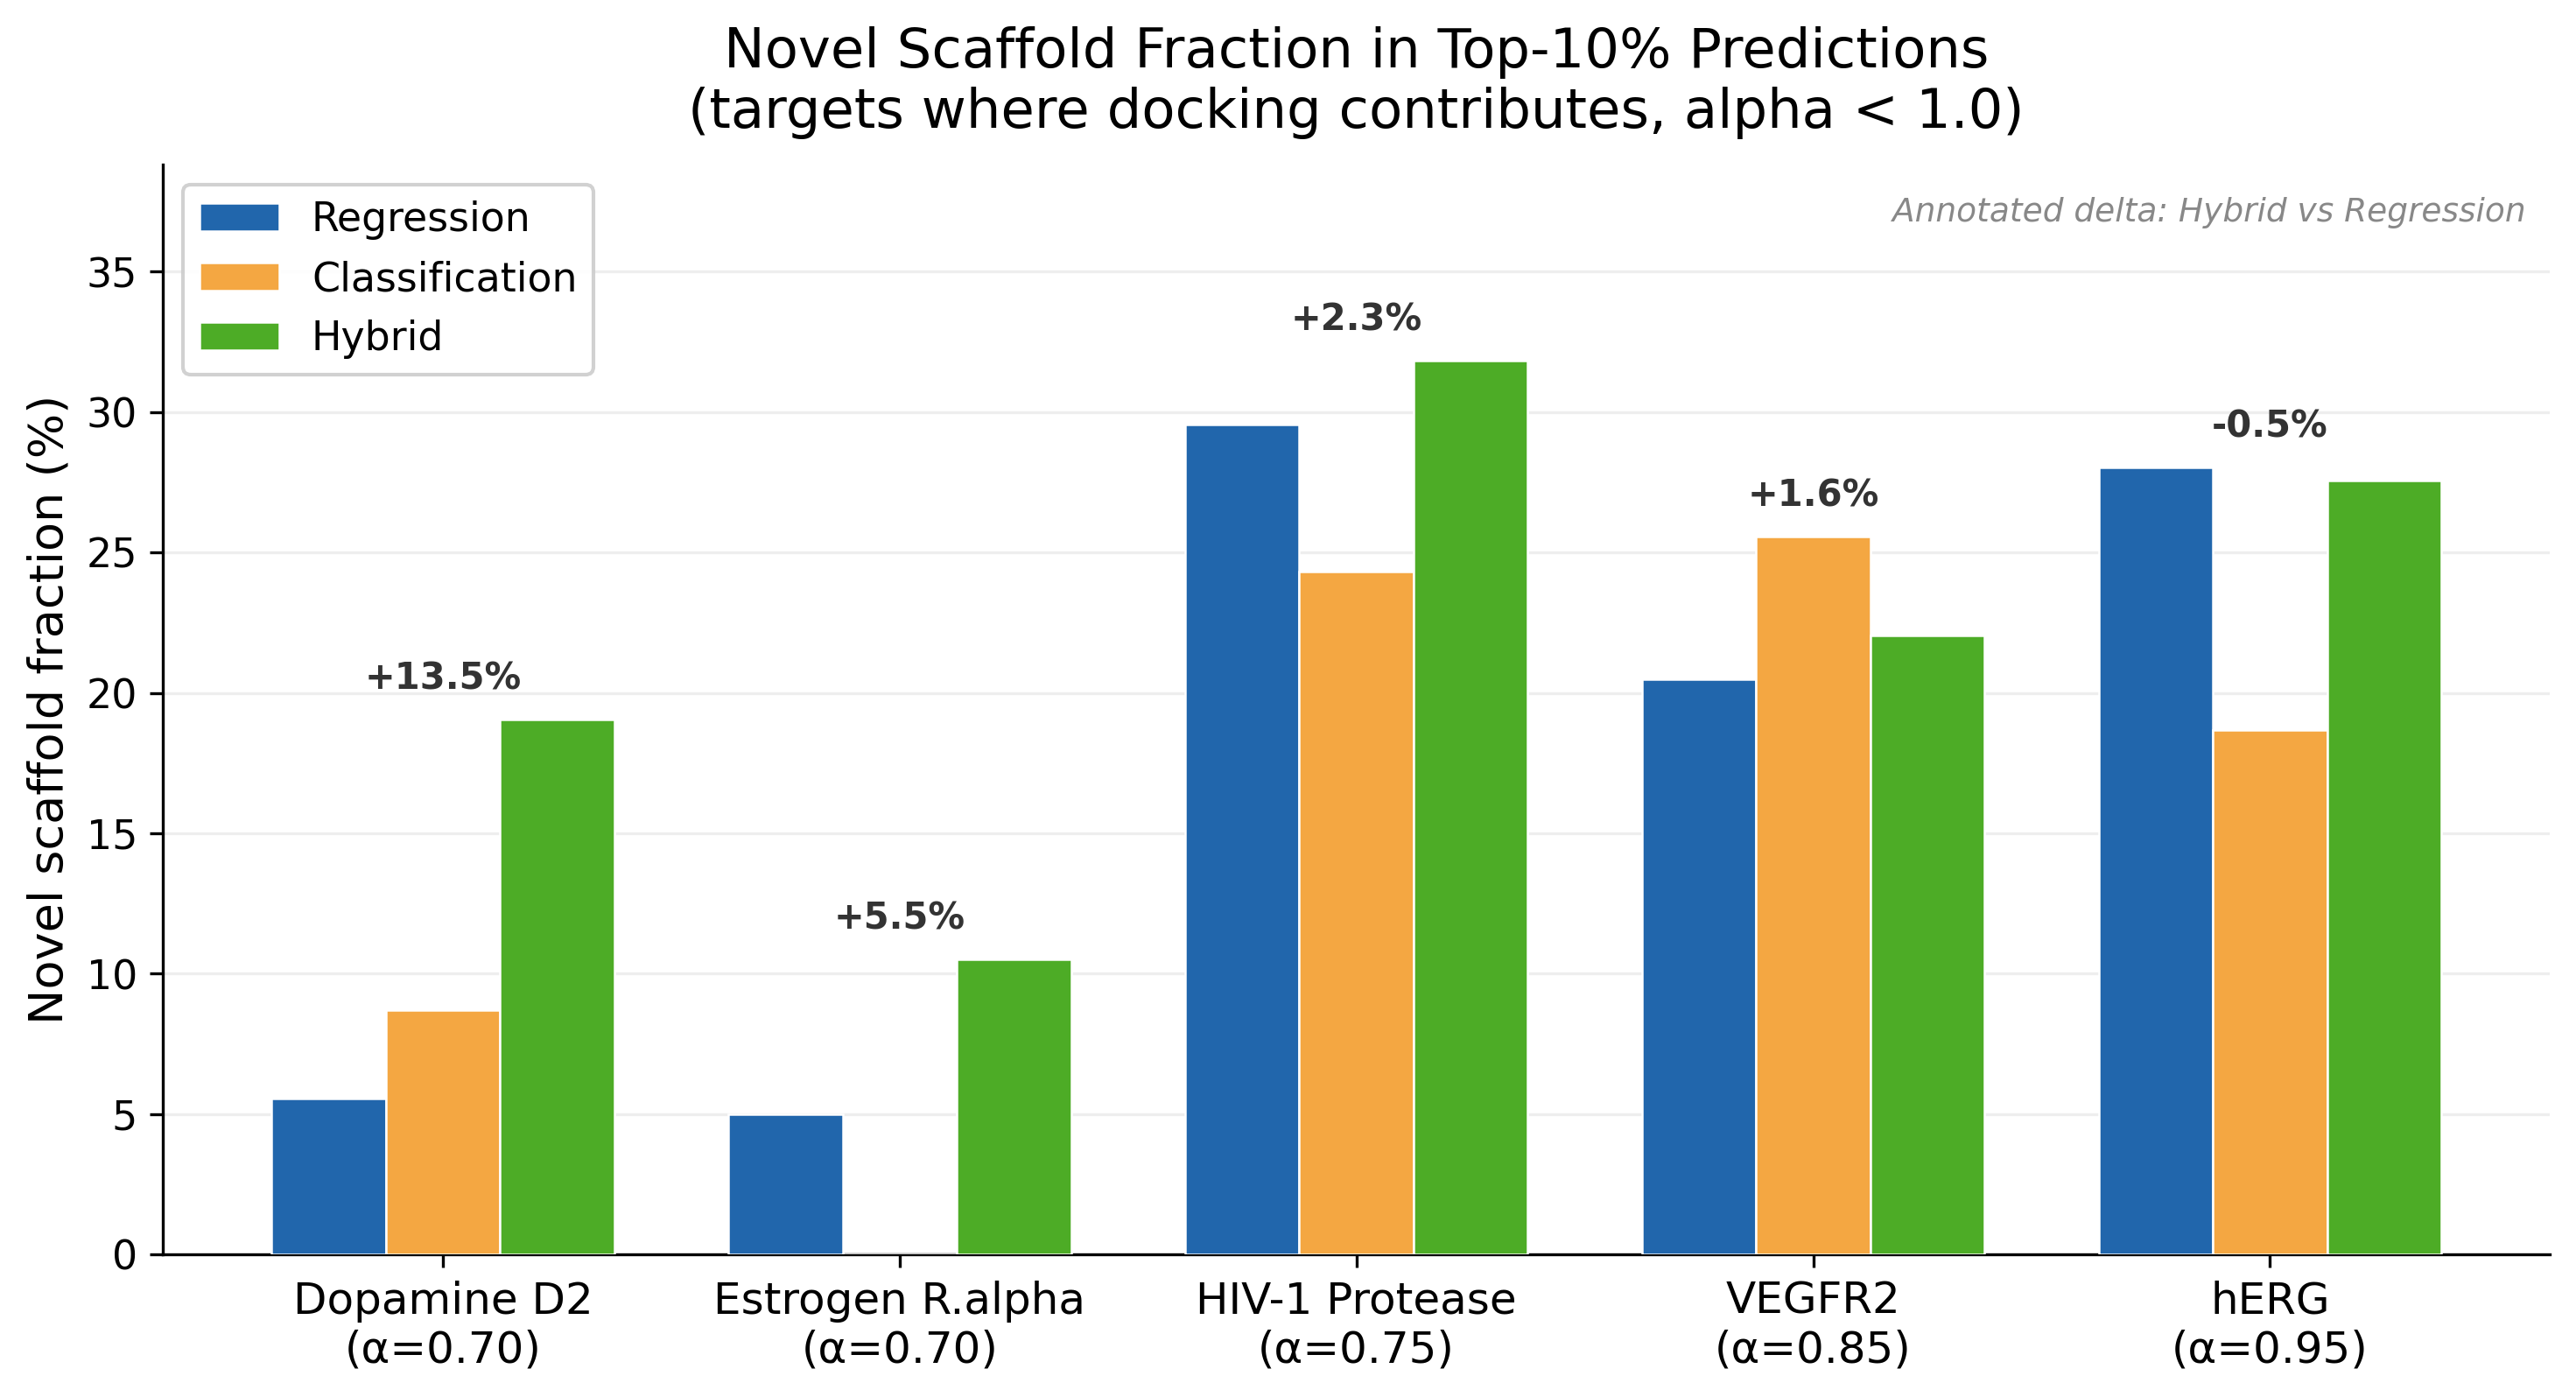
\includegraphics[width=\linewidth]{images/fig_E1_scaffold_diversity.png}
\caption{Novel scaffold fraction in top-10\% predictions
for targets where docking contributes ($\alpha{<}1.0$).
Mean novel fraction increases from 17.7\% (regression)
to 22.2\% (hybrid), a ${\sim}25\%$ relative gain.
Dopamine~D$_2$ shows the strongest improvement
($+13.5$~pp).}
\label{fig:scaffold}
\end{figure}

Hybrid scoring increases mean novel scaffold fraction
from 17.7\% to 22.2\% (${\sim}25\%$ relative gain)
for targets where docking contributes a genuine
structural signal.
The strongest effect is Dopamine~D$_2$ ($+13.5$~pp,
from 5.6\% to 19.0\%), where docking identifies
structurally distinct binders that the ligand-based
model alone misses.
hERG shows negligible change ($-0.5\%$), consistent
with its near-unity $\alpha{=}0.95$.
These results confirm that hybrid consensus expands
chemical space exploration for rigid-pocket targets,
a practically relevant property for scaffold-diverse
hit-to-lead campaigns.


%%% ============================================================
%%% V-K  DUD-E EXTERNAL VALIDATION  →  TABLE
%%% ============================================================
\subsection{\textbf{DUD-E External Validation}}
\label{sec:dude-results}

\begin{table}[!htbp]
\centering
\caption{DUD-E external transfer benchmark. Models trained on ChEMBL data; DUD-E actives scored out-of-distribution. $\alpha$ values are optimised on DUD-E data (upper-bound estimates).}
\label{tab:dude}
\scalebox{0.68}{
\begin{tabular}{llcrrrrr}
\toprule
\textbf{DUD-E} & \textbf{Target} & \textbf{$N_{\mathrm{act}}$} & \textbf{$\alpha$} & \textbf{Reg} & \textbf{Clf} & \textbf{Hyb} & \textbf{NN Tan.} \\
 & & & & \textbf{BEDROC} & \textbf{BEDROC} & \textbf{BEDROC} & \textbf{mean} \\
\midrule
hivpr & HIV-1 Protease & 536 & 0.95 & 0.906 & 0.927 & 0.908 & 0.732 \\
vgfr2 & VEGFR2 & 409 & 0.95 & 0.983 & 0.982 & 0.983 & 0.895 \\
aa2ar & Adenosine A$_{2a}$ & 482 & 0.85 & 0.907 & 0.939 & 0.911 & 0.457 \\
esr1 & ER$\alpha$ & 383 & 0.15 & 0.000 & 0.000 & 0.383 & 0.259 \\
pparg & PPAR$\gamma$ & 484 & 0.00 & 0.000 & 0.000 & 0.000 & 0.255 \\
\bottomrule
\end{tabular}}
\end{table}


Table~\ref{tab:dude} presents out-of-distribution
performance on five DUD-E targets scored by
ChEMBL-trained models.

Performance correlates near-monotonically with
nearest-neighbour Tanimoto similarity between DUD-E
actives and ChEMBL training compounds: hivpr and vgfr2
(NN Tanimoto~$>0.7$) transfer strongly
(BEDROC~$>0.90$); aa2ar (0.457) transfers moderately;
esr1 and pparg ($<0.26$) fail entirely for ligand-based
models.
For esr1, the hybrid score rescues performance from
BEDROC~$0.000$ to $0.383$ at $\alpha{=}0.15$ (85\%
docking weight), demonstrating structure-based recovery
when ligand-based models fall completely outside their
applicability domain.
The pparg total failure reflects both poor chemical
overlap and rigid-receptor limitations for PPAR$\gamma$'s
large, flexible ligand-binding domain
(${\sim}1{,}300$~\AA$^3$).

\textcolor{black}{\subsection{\textbf{ Generalization Beyond Virtual Screening}}
\label{sec:generalization}
Although demonstrated on virtual compound screening, the
framework is domain-agnostic. It applies to any scientific
workload satisfying three requirements: (i)~inference is
deterministic within a pinned runtime configuration, so
outputs are bit-for-bit reproducible (Section~\ref{sec:onnx-results});
(ii)~outputs admit a canonical, order-stable serialization,
so a stable cryptographic digest can be computed; and
(iii)~a permissioned ledger is available to anchor digests
for independent verification. The drug-discovery pipeline
exercises all three, but the same infrastructure transfers
directly to other edge-oriented scientific settings---for
example, environmental IoT sensor analytics, industrial
predictive-maintenance inference, medical edge signal
classification (e.g.\ ECG/EEG), and agricultural
phenotyping---wherever results must be reproduced and
audited across heterogeneous nodes. The classical-ML models
used here are a deliberate consequence of requirement~(i):
they trade the headline accuracy of GPU deep learning for
the bitwise determinism the verification layer depends on
(Section~\ref{sec:ai}), a trade-off appropriate whenever
auditability is the priority.}


%%% ============================================================
%%% V-L  DISCUSSION AND LIMITATIONS
%%% ============================================================
\subsection{\textbf{Limitations}}
\label{sec:discussion}

PureProtX demonstrates that deterministic, cryptographically verifiable
computation is achievable at IoT edge scale without prohibitive overhead.
Merkle batch anchoring reduces per-record provenance cost to 21 ms at
N=100 (< 0.01\% overhead), making cryptographic auditability essentially
free at realistic batch deployment scales. \textcolor{black}{Measured on real
ARM hardware, the full pipeline runs within the memory of a Raspberry Pi~4
for all targets, and inference is bitwise-deterministic within a pinned
runtime configuration across three CPU architectures (Section~V-F), with the
two characterized exceptions noted there.}

Several limitations should be noted. \textcolor{black}{First, throughput
differs measurably across devices---the Raspberry Pi~4 sustains roughly
two-fifths of server throughput (Section~V-A)---so latency-sensitive
deployments must size hardware to the target batch rate; this is a
performance boundary rather than a correctness one, as all tested devices
completed every target without failure.} Second, the MQTT bridge's
sequential commit queue limits throughput to $\sim$20 compounds/s;
Merkle-batched async commits are the path to order-of-magnitude improvement.
Third, \textcolor{black}{validator fault tolerance is now characterised
empirically through controlled failure injection on a
four-signer permissioned testnet
(Section~\ref{sec:consensus-results}): the network
maintains liveness under a single-signer fault, stalls
only on loss of signing majority, and recovers within
$1.04$~s on signer restart. Live failure-injection on the
production PureChain deployment, and validation at larger
signer-set sizes, remain future work.}
Fourth, \textcolor{black}{the present evaluation spans $71{,}853$~compounds;
scaling to ultra-large libraries ($>10^6$~compounds) is
not yet demonstrated. Merkle batch anchoring already
removes the per-record on-chain bottleneck
(Section~\ref{sec:scalability-results}), so the remaining
requirement is distributed inference across multiple edge
nodes---a direct extension of the consortium topology in
Section~\ref{sec:iot-arch} that we leave to future work.}
Fifth, the rigid-receptor docking protocol cannot
capture induced-fit effects, as shown by PPAR$\gamma$
and HIV-1~RT failures.
Sixth, classical ML determinism, while suited to the
framework's cryptographic requirements, may underperform
deep learning where GPU non-determinism is acceptable.


 
%% ============================================================
%%  SECTION VI — CONCLUSION
%%  IEEE Internet of Things Journal — PureProtX
%% ============================================================

\section{\textbf{conclusion}}
\label{sec:conclusion}

This paper presented PureProtX, a deterministic,
blockchain-audited computation framework for IoT-distributed
scientific screening, evaluated across 10~protein targets
spanning 8~protein families (71{,}853~compounds).
The framework addresses a fundamental gap in distributed
IoT scientific pipelines: ensuring that inference results
across heterogeneous edge nodes are provably identical,
tamper-evident, and independently verifiable.
Merkle batch anchoring reduces per-record blockchain overhead
94-fold at $N{=}100$ (21~ms vs.\ ${\sim}2{,}000$~ms for
individual commits), making cryptographic provenance
negligible at realistic deployment scales.
\textcolor{black}{The pipeline runs on real ARM edge hardware,
and inference is bitwise-deterministic within a pinned
runtime configuration---empirically byte-identical across
ONNX Runtime 1.17--1.22, the NumPy 1.26$\rightarrow$2.5
boundary, and three CPU architectures for six of seven
models, with the RBF-kernel SVR the sole
architecture-dependent exception---while all model and result
hashes are anchored on PureChain.}
On the screening workload, the dual consensus ensemble
achieves mean $R^2{=}0.693$, AUC-ROC~$=0.937$, and
BSS~$=0.577$, with docking contributing meaningfully only
for rigid binding pockets where it increases scaffold
novelty by ${\sim}25\%$ and the LOTO default
$\alpha{=}0.935{\pm}0.039$ providing principled hybrid
scoring for novel targets without per-target optimisation.

Several directions for future work emerge from these
findings.
Asynchronous Merkle-batched MQTT commits would eliminate
the sequential blockchain bottleneck for high-frequency
IoT deployments.
\textcolor{black}{Having validated the gap-condition mechanism through
controlled failure injection on a permissioned testnet
(Section~\ref{sec:consensus-results}), a natural next step
is failure-injection on the production deployment and at
larger signer-set sizes to confirm the recovery envelope
at scale.}
Scaling to ultra-large libraries ($>10^6$~compounds) will
require distributed inference and batch-optimised
blockchain commitment.
Integration with FAIR-compliant data catalogues and
decentralised validator networks would broaden data
accessibility and trust assumptions for multi-institutional,
regulatory-ready deployment.

\sloppy
\section*{\textbf{data availability}}

All source code, curated datasets, trained model artefacts,
ONNX exports, deterministic JSON outputs, Docker environment
files, experiment reproduction scripts, and a standalone
on-chain verification tool
(\texttt{tools/verify\_onchain.py}) are publicly available
at \url{https://github.com/xaviwho/PureProt/tree/iot-reframing}.
The repository includes version-pinned dependencies
(Python~3.12.10, scikit-learn~1.8, RDKit~2025.9.4,
AutoDock Vina~1.2.7), pre-configured PureChain test wallet
credentials for immediate blockchain verification
(Chain~ID~900520900520,
Contract~\texttt{\mbox{0xb8eb74663c1297825b188D8454a469d02Cc7d56C}}),
and a single-command reproduction entry point
(\texttt{python experiments/run\_experiments.py}).
ChEMBL bioactivity data were obtained from
ChEMBL~v34~\cite{mendez2019chembl} and DUD-E benchmarks
from~\cite{mysinger2012directory}; both are publicly
accessible.


\section *{\textbf{acknowledgment}} 
This work was partly supported by Innovative Human Resource Development for Local Intellectualization program through the IITP grant funded by the Korea government (MSIT) (IITP-2026-RS-2020-II201612, 33\%) and by Priority Research Centers Program through the NRF funded by the MEST (2018R1A6A1A03024003, 33\%) and by the MSIT, Korea, under the ITRC support program (IITP-2026-RS-2024-00438430, 34\%).

\balance

\bibliographystyle{IEEEtran}
\bibliography{newref,Bibliography}

\end{document}

